\documentclass[12pt,a4paper]{article}

% ─── Packages ─────────────────────────────────────────────────────────────
\usepackage[utf8]{inputenc}
\usepackage[T1]{fontenc}
\usepackage{amsmath,amssymb,amsthm}
\usepackage{mathtools}
\usepackage[margin=1in]{geometry}
\usepackage{hyperref}
\usepackage{xcolor}
\usepackage{booktabs}
\usepackage{longtable}
\usepackage{enumitem}
\usepackage{fancyhdr}
\usepackage{graphicx}
% Gracefully handle missing figure files (e.g. when building on a machine
% where results/images/presentation/ has not been synced). If the file is
% present, render at the requested size; if not, show a framed placeholder
% so the build still succeeds.
\let\origincludegraphics\includegraphics
\renewcommand{\includegraphics}[2][]{%
  \IfFileExists{#2}{\origincludegraphics[#1]{#2}}{%
    \IfFileExists{figures/#2}{\origincludegraphics[#1]{figures/#2}}{%
      \fbox{\parbox{0.6\linewidth}{\centering\textit{figure not available in build environment:}\\\detokenize{#2}}}}}}
\usepackage{float}
\usepackage{listings}
\usepackage[textsize=footnotesize,textwidth=2.2cm,disable]{todonotes}
\usepackage{tcolorbox}
\usepackage{tikz}
\usetikzlibrary{arrows.meta,positioning,shapes.geometric,calc}

% Path to presentation figures
\graphicspath{{figures/}}

% ─── Custom commands (replacing physics package) ──────────────────────────
\newcommand{\abs}[1]{\left|#1\right|}
\newcommand{\norm}[1]{\left\|#1\right\|}
\newcommand{\pdv}[2]{\frac{\partial #1}{\partial #2}}
\newcommand{\dv}[2]{\frac{d #1}{d #2}}
\newcommand{\Real}{\operatorname{Re}}
\newcommand{\Imag}{\operatorname{Im}}
\newcommand{\Tr}{\operatorname{Tr}}
\newcommand{\FFT}{\operatorname{FFT}}
\newcommand{\IFFT}{\operatorname{IFFT}}
\DeclareMathOperator{\sech}{sech}
\DeclareMathOperator{\acosh}{acosh}
\DeclareMathOperator{\sign}{sign}
\DeclareMathOperator{\diag}{diag}

% ─── Julia listings setup ─────────────────────────────────────────────────
\definecolor{jlstring}{RGB}{42,161,152}
\definecolor{jlkeyword}{RGB}{133,153,0}
\definecolor{jlcomment}{RGB}{147,161,161}
\definecolor{jlbackground}{RGB}{253,246,227}
\definecolor{jltype}{RGB}{38,139,210}

\lstdefinelanguage{Julia}{
  keywords={function, end, if, else, elseif, for, while, return, begin, let, do, in, using, import, export, module, struct, mutable, abstract, type, const, true, false, nothing, try, catch, finally, break, continue, macro, quote, local, global},
  keywordstyle=\color{jlkeyword}\bfseries,
  ndkeywords={ComplexF64, Float64, Int, Dict, Vector, Matrix, Array, Nothing, Bool, String, Symbol, Tuple, NamedTuple},
  ndkeywordstyle=\color{jltype},
  sensitive=true,
  comment=[l]{\#},
  commentstyle=\color{jlcomment}\itshape,
  stringstyle=\color{jlstring},
  string=[b]",
  morestring=[b]',
  showstringspaces=false,
  backgroundcolor=\color{jlbackground},
  basicstyle=\ttfamily\footnotesize,
  breaklines=true,
  frame=single,
  rulecolor=\color{black!30},
  numbers=left,
  numberstyle=\tiny\color{gray},
  numbersep=5pt,
  tabsize=4,
  columns=flexible,
  literate={ũ}{{\~{u}}}1 {λ̃}{{\~{$\lambda$}}}1 {φ}{$\varphi$}1 {Δ}{$\Delta$}1
           {≠}{$\neq$}1 {≤}{$\leq$}1 {≥}{$\geq$}1 {∂}{$\partial$}1
           {√}{$\sqrt{}$}1 {π}{$\pi$}1 {ε}{$\varepsilon$}1,
}
\lstset{language=Julia}

% ─── Header/Footer ────────────────────────────────────────────────────────
\pagestyle{fancy}
\fancyhf{}
\fancyhead[L]{\small Rivera Lab --- Raman Suppression Verification}
\fancyhead[R]{\small\thepage}
\fancyfoot[C]{\small Independent Analytical Verification --- \today}

% ─── Theorem environments ─────────────────────────────────────────────────
\theoremstyle{definition}
\newtheorem{finding}{Finding}[section]
\newtheorem{concern}{Concern}[section]

% ─── Colored boxes ────────────────────────────────────────────────────────
\newtcolorbox{verified}{colback=green!5,colframe=green!50!black,title=\textbf{Verified Correct}}
\newtcolorbox{flagged}{colback=red!5,colframe=red!50!black,title=\textbf{Issue Found}}
\newtcolorbox{advisory}{colback=yellow!5,colframe=yellow!50!black,title=\textbf{Advisory Note}}
\newtcolorbox{keyresult}{colback=blue!5,colframe=blue!50!black,title=\textbf{Key Result}}

% ═════════════════════════════════════════════════════════════════════════
\title{\textbf{Independent Analytical Verification of\\
Adjoint-Based Spectral Phase Optimization\\
for Raman Suppression in Optical Fiber}\\[12pt]
\large MultiModeNoise.jl / smf-gain-noise Repository\\
Rivera Lab, Cornell University}
\author{Verification Document Prepared for Ignacio Rivera\\
\small Cornell University, Department of Physics}
\date{March 2026 --- v3 (updated 2026-04-02: line numbers, adjoint solver, log-cost, Raman overflow fix, diagrams, data figures)}

\begin{document}
\maketitle
\thispagestyle{empty}

\begin{abstract}
This document presents an independent, equation-by-equation verification of the mathematical formulation and Julia implementation of an adjoint-based spectral phase optimization system for Raman suppression in single-mode optical fiber. We re-derive every key equation from first principles, audit the source code in the \texttt{smf-gain-noise/} repository against these derivations, and assess whether the overall research approach is sound. The verification covers: (1)~the forward Generalized Nonlinear Schr\"odinger Equation (GNLSE) in the interaction picture, (2)~the cost function and its Wirtinger derivative, (3)~the adjoint equation for reverse-mode sensitivity analysis, (4)~the chain rule through the spectral phase mask, (5)~the regularization terms and their gradients, and (6)~the numerical methods and validation tests. We find that \textbf{the core mathematical formulation is correct}, with the adjoint gradient verified to $0.026\%$ relative error against finite differences. The original cost/gradient scale bug is now resolved via the log-scale objective with the proper chain-rule factor; the main remaining open concern in the single-mode path is the forward attenuator not being carried through the adjoint exactly. Additional advisory items concern regularization interpretation and the physical realizability of some optimized phase profiles.
\medskip\noindent\textbf{v3 update (2026-04-02):} All 13 stale line numbers re-verified. Adjoint solver updated from Vern9/1e-10 to Tsit5/1e-8. Added: log-scale cost function (Section~\ref{sec:new_infra}), Raman response overflow fix, auto-sizing time windows, boundary verification results, TikZ diagrams, and sweep result figures. SPM formula corrected (was missing 0.86/$T_0$ factor).
\end{abstract}

\tableofcontents
\newpage

% ═════════════════════════════════════════════════════════════════════════
\section{Introduction and Research Context}
\label{sec:intro}

% ─── 1.1 What is Raman scattering? ──────────────────────────────────────
\subsection{Stimulated Raman Scattering in Optical Fibers}

When an intense ultrashort laser pulse propagates through an optical fiber, it interacts with the molecular vibrations of the silica glass. This interaction, called \emph{stimulated Raman scattering} (SRS), transfers energy from the pulse (the ``pump'') to longer wavelengths (lower frequencies), creating a ``Stokes'' wave red-shifted by approximately 13~THz from the pump center frequency. The physical mechanism is inelastic scattering: a pump photon is absorbed and re-emitted at lower energy, with the energy difference exciting a vibrational mode of the SiO$_2$ molecule.

For ultrashort pulses ($\sim$100~fs), the Raman effect manifests as the \emph{Raman self-frequency shift} (RSFS): the pulse's spectral center of mass drifts continuously toward longer wavelengths as it propagates. This is particularly important in the anomalous dispersion regime ($\beta_2 < 0$) near 1550~nm, where soliton dynamics amplify the effect. The soliton self-frequency shift, first described by Gordon (1986) and Mitschke and Mollenauer (1986), scales as $T_0^{-4}$ for fundamental solitons, making short pulses especially vulnerable.

\subsection{Why Suppress Raman?}

In many applications---frequency comb generation, supercontinuum sources, quantum noise squeezing experiments (the Rivera Lab's primary interest)---the Raman-shifted energy represents an uncontrolled loss channel. Energy transferred to the Stokes wave is unavailable for the target process. Suppressing Raman scattering while preserving the desired nonlinear interaction (Kerr effect, soliton formation) is therefore a key engineering goal.

\subsection{Spectral Phase Shaping as a Control Knob}

The key physical insight behind this project is that the \emph{spectral phase} $\varphi(\omega)$ applied to the input pulse changes its temporal profile without altering its power spectrum. Different temporal shapes experience different peak power histories during propagation, leading to different amounts of Raman scattering. By optimizing $\varphi(\omega)$, we can search for temporal profiles that minimize Raman energy transfer.

This is physically realizable using standard pulse shaping technology: a spatial light modulator (SLM) in a 4$f$-line can apply arbitrary spectral phases with $\sim$10~mrad precision. The approach has been used extensively in coherent control of chemical reactions and multiphoton microscopy, but its application to Raman suppression in fiber propagation appears to be \textbf{relatively novel}.\todo{Advisor Q: ``Is this actually new?''}

\subsection{Literature Context}

\begin{itemize}[leftmargin=*]
\item \textbf{GNLSE formulation:} The governing equation follows Agrawal, \emph{Nonlinear Fiber Optics}, 6th ed.\ (2019), Chapter~2 (NLSE derivation) and Chapter~13 (Raman response). The Raman response function $h_R(t)$ uses the Blow--Wood model (1989).

\item \textbf{Adjoint methods for the NLSE:} Marcuse (1990) applied perturbation theory to the NLSE. More recently, \emph{Adjoint sensitivity analysis approach for the nonlinear Schr\"odinger equation} by Ganapathysubramanian and Zabaras (Optics Letters, 2019) explicitly derived adjoint-based gradients for NLSE optimization in fiber optics. The mathematical framework---Lagrange multipliers enforcing the PDE constraint, backward propagation of the co-state---is standard in PDE-constrained optimization (see Hinze et al., 2009; Tr\"oltzsch, 2010).

\item \textbf{Raman suppression techniques:} Published approaches include spectral filtering via fiber Bragg gratings (Chen et al., Appl.\ Opt.\ 2017), fiber design (large mode area, photonic crystal fibers), and simply using shorter fibers or lower power. Spectral \emph{amplitude} shaping for SRS control has been demonstrated, but spectral \emph{phase} optimization via adjoint methods for Raman suppression appears to be unexplored in the published literature as of 2025.

\item \textbf{L-BFGS for PDE-constrained optimization:} L-BFGS is the default optimizer in major PDE-constrained optimization frameworks (dolfin-adjoint, ADCME). It is well-suited because it requires only gradient evaluations (no Hessian), has low memory footprint via limited-memory updates, and handles large parameter spaces ($N_t \sim 10^4$) efficiently.
\end{itemize}

\begin{advisory}
The novelty of this approach---adjoint-based spectral phase optimization for Raman suppression---is both a strength and a risk. It is a strength because it addresses a real problem with a principled method. It is a risk because the lack of published comparisons means we cannot validate our results against independent implementations. The finite-difference gradient checks and the physical validation tests (soliton propagation, energy conservation, dispersion broadening) are therefore \emph{critical} evidence of correctness.
\end{advisory}


% ═════════════════════════════════════════════════════════════════════════
\section{The Forward Model: Generalized NLSE}
\label{sec:forward}

\subsection{The Lab-Frame GNLSE}

The electric field envelope $u(z,t)$ in a single-mode fiber satisfies the generalized nonlinear Schr\"odinger equation (GNLSE). In the frequency domain, the lab-frame GNLSE is:
\begin{equation}
\pdv{\hat{u}_\omega}{z} = iD(\omega)\hat{u}_\omega + i\gamma\,\hat{S}(\omega)\,\mathcal{F}\!\left[\left(1-f_R\right)|u|^2 u + f_R\left(h_R * |u|^2\right)u\right]
\label{eq:gnlse_lab}
\end{equation}
where:
\begin{itemize}[leftmargin=*]
\item $D(\omega) = \sum_{n=2}^{N_\beta} \frac{\beta_n}{n!}\omega^n$ is the dispersion operator (Taylor expansion of the propagation constant about $\omega_0$). Note: $\beta_0$ (common phase) and $\beta_1$ (group velocity) are excluded---we work in the co-moving frame.
\item $\gamma$ is the nonlinear coefficient [W$^{-1}$m$^{-1}$].
\item $\hat{S}(\omega) = \omega/\omega_0$ is the self-steepening operator.
\item $f_R = 0.18$ is the fractional Raman contribution.
\item $h_R(t)$ is the Raman response function.
\item $*$ denotes temporal convolution.
\item $\mathcal{F}$ denotes the Fourier transform (time $\to$ frequency).
\end{itemize}

\begin{verified}
\textbf{Comparison to Agrawal:} Equation~\eqref{eq:gnlse_lab} matches Agrawal Eq.~(2.3.36) for the case of a single mode ($M=1$). The self-steepening term $S(\omega) = 1 + \omega/\omega_0$ in Agrawal's notation reduces to $\omega/\omega_0$ when the ``1'' is absorbed into the overall structure of the equation (the ``1'' corresponds to the standard NLSE without self-steepening; the code implements the full ratio $\omega/\omega_0$, which is equivalent for frequencies near $\omega_0$). The Raman response uses the Blow--Wood model, consistent with Agrawal Eq.~(2.3.40).
\end{verified}

\subsection{The Interaction Picture}
\label{sec:interaction_picture}

The dispersion term $iD(\omega)\hat{u}_\omega$ is \emph{stiff}: it produces rapid oscillations in $\hat{u}_\omega$ without changing the pulse shape. We remove it via the transformation:
\begin{equation}
\boxed{\tilde{u}_\omega(z) = e^{-iD(\omega)z}\,\hat{u}_\omega(z)}
\label{eq:interaction_picture}
\end{equation}
This is the \emph{interaction picture}, analogous to the interaction picture in quantum mechanics. Substituting:
\begin{align}
\pdv{\tilde{u}_\omega}{z} &= -iD(\omega)\tilde{u}_\omega + e^{-iD(\omega)z}\pdv{\hat{u}_\omega}{z} \nonumber\\
&= -iD(\omega)\tilde{u}_\omega + e^{-iD(\omega)z}\left[iD(\omega)\hat{u}_\omega + i\gamma\hat{S}(\omega)\mathcal{F}[\text{NL}]\right] \nonumber\\
&= e^{-iD(\omega)z}\cdot i\gamma\hat{S}(\omega)\cdot\mathcal{F}[\text{NL}]
\label{eq:ip_ode}
\end{align}
where $\text{NL} = (1-f_R)|u|^2 u + f_R(h_R*|u|^2)u$ is evaluated using the lab-frame field $\hat{u}_\omega = e^{iD(\omega)z}\tilde{u}_\omega$.

\begin{keyresult}
The interaction picture ODE for the GNLSE (single mode, $M=1$):
\begin{equation}
\boxed{\dv{\tilde{u}_\omega}{z} = i\,e^{-iD(\omega)z}\cdot\hat{S}(\omega)\cdot\mathcal{F}\!\left[\gamma(1-f_R)|u|^2 u + \gamma(h_R*|u|^2)u\right]}
\label{eq:forward_ode}
\end{equation}
where $u(z,t) = \mathcal{F}^{-1}[e^{iD(\omega)z}\tilde{u}_\omega(z)]$ is the lab-frame time-domain field.
\end{keyresult}

\subsection{Code Implementation of the Forward RHS}

The function \texttt{disp\_mmf!} in \texttt{simulate\_disp\_mmf.jl} implements Eq.~\eqref{eq:forward_ode}. The computational steps are:

\begin{enumerate}[leftmargin=*]
\item \textbf{Lines 28--29:} Compute $e^{\pm iD(\omega)z}$:
\begin{lstlisting}
@. exp_D_p = cis(Dw * z)    # exp(+iDz)
@. exp_D_m = cis(-Dw * z)   # exp(-iDz)
\end{lstlisting}

\item \textbf{Line 31:} Transform to lab frame: $\hat{u}_\omega = e^{iDz}\tilde{u}_\omega$:
\begin{lstlisting}
@. uw = exp_D_p * uw_tilde
\end{lstlisting}

\item \textbf{Lines 33--36:} Transform to time domain and extract real/imaginary parts:
\begin{lstlisting}
fft_plan_M! * uw      # FFT: freq -> time (in this convention)
@. ut = attenuator * uw
@. v = real(ut)
@. w = imag(ut)
\end{lstlisting}

\textbf{Convention note:} The code uses $u_\omega = \IFFT(u_t)$, so $u_t = \FFT(u_\omega)$. This is an \emph{inverted} convention compared to the standard physics convention where $\hat{u} = \FFT(u)$.

\item \textbf{Lines 39--43:} Compute Kerr nonlinearity $\eta_K = (1-f_R)\gamma|u|^2 u$:
\begin{lstlisting}
@tullio dKt[t,i,j] = g[i,j,k,l] * (v[t,k]*v[t,l] + w[t,k]*w[t,l])
@tullio aK[t,i] = dKt[t,i,j] * v[t,j]
@tullio bK[t,i] = dKt[t,i,j] * w[t,j]
@. hKt = aK + 1im * bK
@. hKt *= one_m_fR
\end{lstlisting}

For $M=1$: $\delta_K = \gamma(v^2 + w^2) = \gamma|u|^2$, and $\eta_K = \delta_K \cdot u \cdot (1-f_R) = (1-f_R)\gamma|u|^2 u$. \textbf{Correct.}

\item \textbf{Lines 46--54:} Compute Raman nonlinearity $\eta_R = \gamma(h_R * |u|^2)u$ via FFT convolution:
\begin{lstlisting}
@. dKt_cplx = ComplexF64(dKt, 0.0)  # |u|^2 as complex
fft_plan_MM! * dKt_cplx              # FFT(|u|^2)
@. hRw_dRw = hRw * dKt_cplx         # h_R(w) * FFT(|u|^2)
ifft_plan_MM! * hRw_dRw              # IFFT -> time domain
fftshift!(hR_conv_dR, hRw_dRw, 1)   # correct time ordering
@. dRt = real(hR_conv_dR)            # h_R * |u|^2 (real)
\end{lstlisting}

The convolution theorem gives $h_R * |u|^2 = \IFFT[\hat{h}_R \cdot \FFT[|u|^2]]$. The \texttt{fftshift!} on line~50 corrects for the fact that both $h_R(t)$ and $|u(t)|^2$ are stored in centered time ordering (symmetric about $t=0$), and circular convolution of centered arrays requires an \texttt{fftshift} of the output.

\item \textbf{Lines 57--60:} Combine, apply self-steepening, and transform to interaction picture:
\begin{lstlisting}
@. ht = hKt + hRt             # total NL in time domain
ifft_plan_M! * ht              # to frequency domain
ht .*= selfsteep               # multiply by w/w0
@. duw_tilde = 1im * exp_D_m * ht  # interaction picture
\end{lstlisting}

The self-steepening factor \texttt{selfsteep = fftshift($\omega_s / \omega_0$)} is in FFT order (double-fftshifted from the construction in \texttt{get\_p\_disp\_mmf}, line~97). After IFFT, the nonlinear response is also in FFT order. So the element-wise multiplication is correct.
\end{enumerate}

\begin{verified}
The forward solver correctly implements Eq.~\eqref{eq:forward_ode}. The sequence of operations---lab frame recovery, time-domain nonlinear computation, FFT convolution for Raman, frequency-domain self-steepening, interaction picture projection---matches the mathematical formulation.
\end{verified}

\begin{flagged}
\textbf{Attenuator during propagation (line 21):} The code applies \texttt{attenuator} (a super-Gaussian temporal window) to the time-domain field \emph{during} the ODE solve, not just as a diagnostic. This modifies the physical dynamics by absorbing energy at the temporal window edges. The attenuator is \textbf{not included in the adjoint equation}, creating a potential gradient inconsistency. However, the attenuator is essentially unity ($>0.9999$) for $|t| < 0.85 \times T_{\text{window}}/2$, so the error is negligible when the pulse stays well within the window. The boundary penalty in the optimization ensures this condition holds. \textbf{Recommendation:} Log the maximum attenuator-induced energy loss per propagation step. If it exceeds $10^{-6}$, the gradient is unreliable.
\end{flagged}

\subsection{Dispersion Operator Construction}

In \texttt{helpers.jl}, line~187 (in \texttt{get\_disp\_fiber\_params\_user\_defined}):
\begin{equation}
D[\omega_k] = \sum_{n=0}^{N_\beta} \frac{\beta_n}{n!}\left(2\pi f_k \times 10^{12}\right)^n
\label{eq:dispersion_discrete}
\end{equation}
where $f_k = \texttt{fftfreq}(N_t, 1/\Delta t)$ in THz. The factor $10^{12}$ converts THz to Hz for compatibility with $\beta_n$ in SI units (s$^n$/m).

\begin{verified}
The $\beta_n$ vector (line~180) is constructed as $[\beta_0, \beta_1, \beta_2, \beta_3, \ldots]$ with $\beta_0 = 0$ and $\beta_1 = 0$. This correctly excludes the common phase and group velocity terms, placing us in the co-moving frame.
\end{verified}

\subsection{Raman Response Function}

The Blow--Wood model:
\begin{equation}
h_R(t) = f_R \cdot \frac{\tau_1^2 + \tau_2^2}{\tau_1\tau_2^2}\exp\!\left(-\frac{t}{\tau_2}\right)\sin\!\left(\frac{t}{\tau_1}\right)\Theta(t)
\label{eq:raman_response}
\end{equation}

The discrete version (\texttt{helpers.jl}, line~182 in \texttt{get\_disp\_fiber\_params\_user\_defined}, or line~107 in \texttt{get\_disp\_fiber\_params}) includes a factor $\Delta t \times 10^3$ and a numerical overflow fix:
\begin{equation}
h_R[n] = f_R \cdot \Delta t_{\text{ps}} \cdot 10^3 \cdot \frac{\tau_1^2 + \tau_2^2}{\tau_1\tau_2^2}\exp\!\left(-\frac{\max(t_n, 0)}{\tau_2}\right)\sin\!\left(\frac{\max(t_n, 0)}{\tau_1}\right)\Theta(t_n)
\label{eq:raman_discrete}
\end{equation}

\begin{advisory}
\textbf{Overflow fix (v3):} The code uses $\max(t_n, 0)$ inside the exponential to prevent IEEE~754 overflow. For time windows $> 45$~ps, negative time values produce $\exp(|t|/\tau_2) \to +\infty$, and $\infty \times 0 = \text{NaN}$ when multiplied by $\Theta(t_n) = 0$. The $\max$ clamp does not change the mathematical result (since $\Theta$ zeroes out $t < 0$ anyway) but prevents NaN propagation. This fix unblocked all L$=$5~m sweep configurations.
\end{advisory}

\textbf{Unit analysis:} The continuous convolution $\int h_R(\tau)|u(t-\tau)|^2\,d\tau$ becomes the discrete sum $\sum_n h_R[n]|u[t-n]|^2$. To convert: the continuous integral has units of [time$^{-1}$]$\cdot$[W]$\cdot$[time] = [W]. The discrete sum needs a factor of $\Delta t$ to approximate the integral. Since $\Delta t$ is in ps and $\tau_1, \tau_2$ are in fs, the factor $\Delta t_{\text{ps}} \times 10^3$ converts $\Delta t$ from ps to fs, matching the fs units of $\tau_1$ and $\tau_2$ in the denominator. The FFT-based convolution then automatically includes this $\Delta t$ factor.

\begin{verified}
The Raman response discretization is correct. The $\Delta t \times 10^3$ factor ensures proper unit conversion for the discrete convolution via FFT. Parameters $f_R = 0.18$, $\tau_1 = 12.2$~fs, $\tau_2 = 32$~fs match the standard Blow--Wood values for fused silica (Agrawal, Table~2.3).
\end{verified}

\subsection{Physical Parameters}

\begin{center}
\begin{tabular}{lll}
\toprule
Parameter & Value & Source/Comment \\
\midrule
$\beta_2$ (SMF-28) & $-2.17\times10^{-26}$ s$^2$/m & $\approx -21.7$ ps$^2$/km, standard at 1550~nm \\
$\beta_3$ (SMF-28) & $1.2\times10^{-40}$ s$^3$/m & $\approx 0.12$ ps$^3$/km \\
$\gamma$ (SMF-28) & $1.1\times10^{-3}$ W$^{-1}$m$^{-1}$ & $\approx 1.1$ (W$\cdot$km)$^{-1}$, standard \\
$\gamma$ (HNLF) & $10.0\times10^{-3}$ W$^{-1}$m$^{-1}$ & Reasonable for HNLF \\
$f_R$ & 0.18 & Standard for silica \\
$\lambda_0$ & 1550 nm & Telecom C-band \\
Pulse FWHM & 185 fs & Sub-200~fs soliton regime \\
Rep rate & 80.5 MHz & Standard mode-locked laser \\
\bottomrule
\end{tabular}
\end{center}

\begin{verified}
All physical parameters are within the expected range for single-mode silica fiber at 1550~nm. The SMF-28 values match Corning specifications. The HNLF values are reasonable for commercial highly nonlinear fiber.
\end{verified}


% ═════════════════════════════════════════════════════════════════════════
\section{The Optimization Problem}
\label{sec:optimization}

\subsection{Decision Variable and Cost Function}

The optimization variable is the spectral phase $\varphi(\omega)$, a real-valued function discretized on the FFT frequency grid ($N_t$ values). The shaped input pulse is:
\begin{equation}
u_0(\omega) = u_{00}(\omega)\,e^{i\varphi(\omega)}
\label{eq:phase_mask}
\end{equation}
where $u_{00}(\omega)$ is the unmodified (transform-limited) pulse spectrum.

The cost function measures the fractional energy in the Raman band:
\begin{equation}
\boxed{J[\varphi] = \frac{E_{\text{band}}}{E_{\text{total}}} = \frac{\sum_{\omega \in \mathcal{B}}|u_L(\omega)|^2}{\sum_\omega |u_L(\omega)|^2}}
\label{eq:cost}
\end{equation}

The Raman band $\mathcal{B}$ is defined as all FFT frequencies with $\Delta f < -5$~THz (Stokes side). In the code (\texttt{common.jl}, line~361):
\begin{lstlisting}
band_mask = Df_fft .< raman_threshold  # raman_threshold = -5.0 THz
\end{lstlisting}

\subsection{Why This Cost Function?}

The ratio $J = E_{\text{band}}/E_{\text{total}}$ is:
\begin{itemize}[leftmargin=*]
\item \textbf{Normalized:} $J \in [0,1]$, independent of total pulse energy.
\item \textbf{Differentiable:} As a ratio of smooth functions of $u_L$, $J$ is differentiable everywhere except where $E_{\text{total}} = 0$ (which never occurs physically).
\item \textbf{Physically meaningful:} $J=0$ means perfect Raman suppression.
\end{itemize}

\begin{advisory}
The band mask is a hard spectral cut at $-5$~THz. This is discontinuous in frequency space, meaning the cost function is non-smooth at the band edges. In practice, the Raman-shifted energy is spread over a broad spectral region, so the exact threshold location is not critical. However, if the optimizer places energy precisely at the threshold, the gradient could be noisy. A smoothed mask (e.g., Fermi function) would be more robust but is not necessary for the current problem.\todo{Consider smoothed mask for future work}
\end{advisory}

\subsection{Why L-BFGS?}

The parameter space has dimension $N_t$ (typically $2^{13}$ to $2^{14}$). The alternatives:
\begin{itemize}[leftmargin=*]
\item \textbf{Grid search / genetic algorithms:} Infeasible for $N_t > 100$.
\item \textbf{Gradient descent:} Converges, but requires careful step-size tuning and has slow convergence for ill-conditioned problems.
\item \textbf{Newton's method:} Requires the Hessian ($N_t \times N_t$ matrix), which is prohibitively expensive.
\item \textbf{L-BFGS:} Approximates the inverse Hessian using the last $m$ gradient pairs (typically $m=10$). Requires only gradient evaluations. Memory cost: $O(mN_t)$. Convergence: superlinear for smooth problems.
\end{itemize}

L-BFGS is the standard choice for large-scale PDE-constrained optimization and is the default in frameworks like dolfin-adjoint.

\subsection{Connection to Machine Learning}

The optimization pipeline is structurally identical to training a neural network:
\begin{center}
\begin{tabular}{lll}
\toprule
ML Concept & This Problem & Key Difference \\
\midrule
Parameters $\theta$ & Phase $\varphi(\omega)$ & Continuous spectral function, not matrix entries \\
Forward pass & GNLSE solve ($z: 0 \to L$) & PDE, not matrix multiplications \\
Loss function & $J = E_{\text{band}}/E_{\text{total}}$ & Physics-based, not cross-entropy \\
Backpropagation & Adjoint solve ($z: L \to 0$) & Continuous adjoint of a PDE \\
Optimizer & L-BFGS & Same as in ML \\
\bottomrule
\end{tabular}
\end{center}

The key difference is that the ``forward model'' is a PDE (with its own truncation errors, stability constraints, and stiffness), not a composition of differentiable layers. This makes the gradient computation more subtle: we need the \emph{continuous adjoint}, not just automatic differentiation through a computation graph.


% ═════════════════════════════════════════════════════════════════════════
\section{The Adjoint Method}
\label{sec:adjoint}

\subsection{Three Perspectives on the Adjoint}

\subsubsection{Perspective 1: Constrained Optimization via Lagrange Multipliers}

We want to minimize $J[u_L]$ subject to the constraint that $u(z)$ satisfies the GNLSE:
\begin{equation}
\dv{u_\omega}{z} = f(u_\omega, z) \quad \text{(the forward ODE)}
\end{equation}

Form the Lagrangian with multiplier $\lambda(z)$:
\begin{equation}
\mathcal{L} = J[u_L] + \int_0^L \left\langle \lambda(z),\, \dv{u}{z} - f(u,z) \right\rangle dz
\label{eq:lagrangian}
\end{equation}

Setting $\delta\mathcal{L}/\delta\lambda = 0$ recovers the forward equation. Setting $\delta\mathcal{L}/\delta u = 0$ gives the \emph{adjoint equation} for $\lambda(z)$, propagating backward from $z=L$ to $z=0$.

\subsubsection{Perspective 2: Continuous Backpropagation}

In a neural network, backpropagation computes $\partial\text{Loss}/\partial\theta_k$ by propagating error signals backward through layers. The adjoint method does the same thing for a continuous ODE: the ``error signal'' $\lambda(z)$ propagates backward through the fiber, accumulating sensitivity information. One backward solve gives the gradient with respect to \emph{all} $N_t$ phase values simultaneously.

\subsubsection{Perspective 3: Computational Cost Argument}

\textbf{Forward sensitivity:} Perturbing each of the $N_t$ phase components requires $N_t$ forward solves $\Rightarrow O(N_t)$ total cost.

\textbf{Finite differences:} Central differences require $2N_t$ forward solves $\Rightarrow O(N_t)$ cost.

\textbf{Adjoint method:} One forward solve + one backward solve $= O(1)$ cost, \emph{independent of $N_t$}.

For $N_t = 8192$, the adjoint method is $\sim$4000$\times$ faster than finite differences. This makes gradient-based optimization feasible.

\subsection{Derivation of the Adjoint Equation}
\label{sec:adjoint_derivation}

For a complex ODE $du/dz = f(u, u^*, z)$, the variation of the cost is:
\begin{equation}
\delta J = 2\Real\sum_\omega \lambda_L^*(\omega)\,\delta u_L(\omega)
\end{equation}
where $\lambda_L = \partial J / \partial u_L^*$ is the terminal condition (derived in the next subsection).

The variation $\delta u_L$ satisfies the \emph{linearized forward equation}. To avoid solving it, we introduce $\lambda(z)$ satisfying the adjoint:
\begin{equation}
\boxed{\dv{\lambda_\omega}{z} = -\left(\pdv{f}{u}\right)^\dagger \lambda - \left(\pdv{f}{u^*}\right)^T \lambda^*}
\label{eq:adjoint_general}
\end{equation}
integrated \emph{backward} from $z=L$ to $z=0$. After integration by parts, the sensitivity reduces to:
\begin{equation}
\delta J = 2\Real\sum_\omega \lambda_0^*(\omega)\,\delta u_0(\omega)
\label{eq:sensitivity}
\end{equation}

\textbf{The factor of 2:} This factor comes from the Wirtinger calculus convention for real-valued cost functions. If $J$ is real and depends on both $u$ and $u^* = \bar{u}$, then:
\begin{equation}
\delta J = \sum_\omega \left(\pdv{J}{u_\omega}\delta u_\omega + \pdv{J}{u_\omega^*}\delta u_\omega^*\right) = 2\Real\sum_\omega \pdv{J}{u_\omega^*}\delta u_\omega
\end{equation}
The second equality uses $(\partial J/\partial u)^* = \partial J/\partial u^*$ for real $J$.

\subsection{Terminal Condition: $\partial J / \partial u_L^*$}
\label{sec:terminal}

We need the Wirtinger derivative of $J = E_{\text{band}}/E_{\text{total}}$ with respect to $u_L^*(\omega)$.

\textbf{Setup:}
\begin{align}
E_{\text{band}} &= \sum_{\omega' \in \mathcal{B}} |u_L(\omega')|^2 = \sum_{\omega'} \mathbb{1}_\mathcal{B}(\omega')\, u_L(\omega')\, u_L^*(\omega') \\
E_{\text{total}} &= \sum_{\omega'} u_L(\omega')\, u_L^*(\omega')
\end{align}

\textbf{Wirtinger derivative:} For a product $u \cdot u^*$:
\begin{equation}
\pdv{(u_{\omega'}u_{\omega'}^*)}{u_\omega^*} = u_{\omega'}\,\delta_{\omega\omega'}
\end{equation}

\textbf{Quotient rule:}
\begin{align}
\pdv{J}{u_\omega^*} &= \frac{1}{E_{\text{total}}}\pdv{E_{\text{band}}}{u_\omega^*} - \frac{E_{\text{band}}}{E_{\text{total}}^2}\pdv{E_{\text{total}}}{u_\omega^*} \nonumber\\
&= \frac{\mathbb{1}_\mathcal{B}(\omega)\,u_L(\omega)}{E_{\text{total}}} - \frac{J\cdot u_L(\omega)}{E_{\text{total}}} \nonumber\\
&= \frac{u_L(\omega)\left[\mathbb{1}_\mathcal{B}(\omega) - J\right]}{E_{\text{total}}}
\end{align}

\begin{keyresult}
The terminal condition for the adjoint:
\begin{equation}
\boxed{\lambda_L(\omega) = \pdv{J}{u_L^*(\omega)} = \frac{u_L(\omega)\left[\mathbb{1}_\mathcal{B}(\omega) - J\right]}{E_{\text{total}}}}
\label{eq:terminal_condition}
\end{equation}
\end{keyresult}

\begin{verified}
Code (\texttt{common.jl}, line~262): \texttt{dJ = uwf .* (band\_mask .- J) ./ E\_total}. This exactly matches Eq.~\eqref{eq:terminal_condition}. The sign, the conjugation pattern, and the normalization are all correct.
\end{verified}

\subsection{Chain Rule Through the Phase Mask}
\label{sec:chain_rule}

From Eq.~\eqref{eq:phase_mask}: $u_0(\omega) = u_{00}(\omega)e^{i\varphi(\omega)}$. A perturbation $\delta\varphi(\omega)$ gives:
\begin{equation}
\delta u_0(\omega) = i\,u_{00}(\omega)e^{i\varphi(\omega)}\,\delta\varphi(\omega) = i\,u_0(\omega)\,\delta\varphi(\omega)
\end{equation}

Substituting into Eq.~\eqref{eq:sensitivity}:
\begin{align}
\delta J &= 2\Real\sum_\omega \lambda_0^*(\omega)\cdot i\,u_0(\omega)\cdot\delta\varphi(\omega) \nonumber\\
\Rightarrow\quad \pdv{J}{\varphi(\omega)} &= 2\Real\!\left[\lambda_0^*(\omega)\cdot i\cdot u_0(\omega)\right]
\end{align}

\begin{keyresult}
\begin{equation}
\boxed{\pdv{J}{\varphi(\omega)} = 2\Real\!\left[\lambda_0^*(\omega)\cdot i\cdot u_0(\omega)\right] = -2\Imag\!\left[\lambda_0^*(\omega)\cdot u_0(\omega)\right]}
\label{eq:gradient_phase}
\end{equation}
\end{keyresult}

\begin{verified}
Code (\texttt{raman\_optimization.jl}, line~90): \texttt{dJ\_dphi = 2.0 .* real.(conj.(l0) .* (1im .* uw0\_shaped))}. This matches Eq.~\eqref{eq:gradient_phase} exactly. The factor of 2 is correctly traced through the Wirtinger convention.
\end{verified}

\textbf{Tracing the factor of 2:} The factor of 2 in Eq.~\eqref{eq:gradient_phase} comes \emph{entirely} from the Wirtinger derivative identity $\delta J = 2\Real\langle \partial J/\partial u^*, \delta u\rangle$ for real-valued $J$. It does \emph{not} appear in the adjoint equation itself or in the terminal condition. The adjoint solver returns $\lambda_0$ without any factor of 2. The factor is applied once, at the very end, in the chain rule step.

\subsection{Interaction Picture for the Adjoint}
\label{sec:adjoint_ip}

\textbf{Claim:} The adjoint variable transforms as $\tilde{\lambda}_\omega = e^{-iD(\omega)z}\lambda_\omega$, the same transformation as the forward field.

\textbf{Proof:} The forward transformation is $u_\omega = M(z)\tilde{u}_\omega$ where $M(z) = e^{iD(\omega)z}$ (diagonal). For the adjoint variable under this coordinate change, we need $\tilde{\lambda}$ such that the inner product is preserved:
\begin{equation}
\langle \lambda, \delta u \rangle = \langle \tilde{\lambda}, \delta \tilde{u} \rangle
\end{equation}

Since $\delta u = M\,\delta\tilde{u}$:
\begin{equation}
\langle \lambda, M\,\delta\tilde{u} \rangle = \langle M^\dagger \lambda, \delta\tilde{u} \rangle
\end{equation}

So $\tilde{\lambda} = M^\dagger \lambda = (e^{iDz})^\dagger \lambda = e^{-iDz}\lambda$ (since $D$ is real diagonal, $M^\dagger = e^{-iDz}$).

\begin{verified}
The transformation $\tilde{\lambda}_\omega = e^{-iD(\omega)z}\lambda_\omega$ is correct. Code (\texttt{sensitivity\_disp\_mmf.jl}, line~168): \texttt{l\_tilde\_wL = exp.(-1im * fiber["Dw"] * fiber["L"]) .* lwL}. This matches.\todo{Advisor Q: ``Why same sign for forward and adjoint?''}
\end{verified}

\subsection{Self-Steepening Adjoint}

The forward equation multiplies the nonlinear response by $\hat{S}(\omega) = \omega/\omega_0$ (real, diagonal in frequency). The adjoint of multiplication by a real diagonal operator $S$ is multiplication by $S^* = S$ (real diagonal operators are self-adjoint). The code (\texttt{sensitivity\_disp\_mmf.jl}, line~24) multiplies $\lambda_\omega$ by \texttt{$\tau_\omega$ = fftshift($\omega_s / \omega_0$)}:

\begin{lstlisting}
lw .*= tw  # self-steepening adjoint
\end{lstlisting}

\begin{verified}
The self-steepening adjoint is correct: multiplication by a real diagonal is self-adjoint.
\end{verified}

\subsection{Raman Convolution Adjoint}

The forward computes $y = h_R * x$ via $\hat{y} = \hat{h}_R \cdot \hat{x}$ (pointwise multiplication in frequency). The adjoint of pointwise multiplication by $\hat{h}_R$ is pointwise multiplication by $\hat{h}_R^*$ (the conjugate).

\textbf{Important:} For real, \emph{causal} $h_R(t)$ (zero for $t<0$), $\hat{h}_R^*(\omega) \neq \hat{h}_R(-\omega)$ in general. The Raman response is real and causal but not symmetric, so $\hat{h}_R^*$ is the correct adjoint, not $\hat{h}_R(-\omega)$.

In the code:
\begin{itemize}[leftmargin=*]
\item Term~3 (\texttt{calc\_$\lambda$\_$\partial$fR2c\_$\partial$uc!}) uses \texttt{hwc = conj(hRw)} $= \hat{h}_R^*$. \textbf{Correct.}
\item Term~4 (\texttt{calc\_$\lambda$c\_$\partial$fR\_$\partial$uc!}) uses \texttt{hw = hRw} $= \hat{h}_R$. \textbf{Correct} (this term involves $\lambda^*$, not $\lambda$, so the conjugation structure is different).
\end{itemize}

\begin{verified}
The Raman convolution adjoint correctly uses $\hat{h}_R^*(\omega)$ (conjugate in frequency) where needed, not $\hat{h}_R(-\omega)$ (time reversal). These differ for the non-symmetric, causal Raman response.
\end{verified}


% ═════════════════════════════════════════════════════════════════════════
\section{Verification of Validation Tests}
\label{sec:validation}

\subsection{Dispersion Broadening Test}

\textbf{What it tests:} Pure linear propagation ($\gamma \to 0$). A Gaussian pulse broadens by the factor $T_{\text{out}}/T_{\text{in}} = \sqrt{1 + (L/L_D)^2}$.

\textbf{Result:} Expected 1.547, measured 1.500 (3\% error).

\textbf{Assessment:} The 3\% discrepancy is likely due to: (a) the test using a sech$^2$ pulse (not Gaussian), for which the broadening formula is approximate; (b) the definition of ``width'' (FWHM vs.\ RMS); (c) higher-order dispersion ($\beta_3$) slightly modifying the broadening. A 10\% tolerance is appropriate for this test. \textbf{PASS---but a more precise test would use a Gaussian pulse with $\beta_3 = 0$ and compare RMS widths.}

\subsection{Soliton Propagation Test}

\textbf{What it tests:} Nonlinear-dispersive balance. A fundamental soliton ($N=1$) should propagate without changing shape when $f_R = 0$.

\textbf{Result:} Shape error 1.3\%, peak power ratio 0.9998.

\textbf{Assessment:} The test uses $f_R \approx 0$ (not exactly zero). Even a small $f_R$ induces a Raman self-frequency shift. For $f_R = 10^{-6}$ and one soliton period, the frequency shift is negligible ($< 10^{-3}$~THz), so this does not explain the 1.3\% shape error. The error is more likely from ODE solver tolerance ($10^{-8}$) and the finite FFT window. \textbf{PASS.}

\subsection{Finite-Difference Gradient Check}

\textbf{What it tests:} The adjoint gradient $\partial J/\partial\varphi$ against $(J(\varphi + \varepsilon e_k) - J(\varphi - \varepsilon e_k))/(2\varepsilon)$ for individual spectral components.

\textbf{Result:} Max relative error 0.026\%.

\textbf{Assessment:} Central finite differences have truncation error $O(\varepsilon^2)$. For $\varepsilon = 10^{-5}$, the expected truncation error is $\sim\varepsilon^2 \cdot |J'''| / 6 \approx 10^{-10}$, much smaller than 0.026\%. The observed error is dominated by the ODE solver tolerance ($10^{-8}$ for forward, $10^{-10}$ for adjoint) and floating-point arithmetic. An error of $2.6 \times 10^{-4}$ is \textbf{excellent} and provides strong evidence of gradient correctness.

\subsection{Taylor Remainder Test}

\textbf{What it tests:} The remainder $r_2(\varepsilon) = |J(\varphi + \varepsilon\delta\varphi) - J(\varphi) - \varepsilon\nabla J \cdot \delta\varphi|$ should be $O(\varepsilon^2)$ if the gradient is correct.

\textbf{Result:} Log-log slopes of 2.00 and 2.04.

\textbf{Assessment:} A slope of exactly 2 confirms second-order convergence. The measured slopes are within floating-point precision of 2.0. This is the \textbf{strongest evidence} that the adjoint gradient is mathematically exact. \textbf{PASS.}

\subsection{Multi-Start Convergence}

\textbf{Result:} 1.52~dB spread across 3 random starting phases after 10 iterations.

\textbf{Assessment:} A 1.52~dB spread after only 10 iterations is not conclusive evidence of either a smooth or rugged landscape. The starts may not have converged. To distinguish local minima from incomplete convergence, run to full convergence (gradient norm $< 10^{-6}$) from $\geq 10$ random starts and compare final costs. If the spread narrows to $< 0.1$~dB, the landscape is likely well-behaved.

\begin{advisory}
The multi-start test as currently implemented (3 starts, 10 iterations) is too weak to draw conclusions about the optimization landscape. Recommend: 10+ starts, run to convergence, report both final costs and optimized phase profiles.
\end{advisory}


% ═════════════════════════════════════════════════════════════════════════
\section{Critical Assessment}
\label{sec:critical}

\subsection{What Is Verified Correct}

\begin{enumerate}[leftmargin=*]
\item \textbf{Forward GNLSE (R1):} The formulation matches Agrawal's standard GNLSE with the Blow--Wood Raman model. The interaction picture transformation, self-steepening, and FFT-based Raman convolution are all correctly implemented. Parameters are physically reasonable.

\item \textbf{Terminal condition (Task 2):} The Wirtinger derivative $\partial J/\partial u_L^*$ is correctly derived and implemented. The quotient rule, the indicator function, and the normalization all match.

\item \textbf{Gradient formula (Task 4):} The chain rule $\partial J/\partial\varphi = 2\Real[\lambda_0^* \cdot i \cdot u_0]$ is correct. The factor of 2 is properly traced through the Wirtinger convention.

\item \textbf{Interaction picture for adjoint (Task 5):} The transformation $\tilde{\lambda} = e^{-iDz}\lambda$ is mathematically correct, proven by inner product preservation.

\item \textbf{Self-steepening adjoint (Task 6):} Real diagonal operators are self-adjoint. Correct.

\item \textbf{Raman adjoint conjugation (Task 7):} Uses $\hat{h}_R^*$ (not $\hat{h}_R(-\omega)$). Correct.

\item \textbf{Raman normalization (Task 8):} The $\Delta t \times 10^3$ factor correctly converts units. Verified.

\item \textbf{Finite-difference gradient validation:} 0.026\% max relative error and Taylor remainder slopes of 2.00/2.04 provide strong evidence of gradient correctness.
\end{enumerate}

\subsection{Issues Found}

\begin{verified}
\textbf{Issue 1: Cost/gradient scale --- RESOLVED in v3 via log-scale cost.} The original bug (v1): \texttt{optimize\_spectral\_phase} returned $10\log_{10}(J)$ (dB) while the gradient was $\partial J/\partial\varphi$ (linear). v2 fix: return linear $J$ directly. v3 approach: intentionally optimize in dB with properly scaled gradient:
\begin{equation}
J_{\text{dB}} = 10\log_{10}(J), \qquad \pdv{J_{\text{dB}}}{\varphi} = \frac{10}{J\ln 10}\cdot\pdv{J}{\varphi}
\end{equation}
The $10/(J\ln 10)$ factor maintains $O(1)$ gradient magnitude as $J \to 0$, preventing L-BFGS stall. Default: \texttt{log\_cost=true}, \texttt{f\_abstol=0.01}~dB.

\textbf{Historical vs.\ current-methodology result.} The \emph{20--28\,dB
improvement} reported in earlier revisions was measured against the pre-fix
run where the vanishing linear-cost gradient numerically stalled L-BFGS (0/10
multistart starts reached convergence). That headline is a fix-vs-broken
comparison, not a methodology comparison. The current-methodology head-to-head,
run as Phase~16's cost-function audit (\texttt{.planning/notes/cost-function-default.md},
\texttt{results/cost\_audit/A/}), reports on SMF-28 $L=0.5$~m $P=0.05$~W (Config~A):
\texttt{log\_dB} reaches $-75.8$\,dB in 10.6\,s (15 iter); correctly-scaled
\texttt{linear} reaches $-70.5$\,dB in 17\,s (10 iter). The gap is therefore
$\approx 5$\,dB at Config~A (7/12 variant runs; Config~C unfinished). The
recommendation to default to \texttt{log\_dB} stands; the physical size of
the improvement in production is $\sim$5\,dB, not $\sim$25\,dB.
\end{verified}

\begin{advisory}
\textbf{New (v4): Landscape is saddle-dominated at canonical L-BFGS optima.}
Phase~13 measured the top-20 and bottom-20 Hessian eigenvalues via
matrix-free Lanczos at SMF-28 ($L=2$\,m, $P=0.2$\,W) and HNLF ($L=0.5$\,m,
$P=0.01$\,W) canonical optima. Both spectra are \emph{indefinite}, with all
20 top eigenvalues positive and all 20 bottom eigenvalues negative:
\begin{center}
\small
\begin{tabular}{lcc}
\toprule
Config & $|\lambda_\text{min}|/\lambda_\text{max}$ & Sign pattern \\
\midrule
SMF-28 canonical & $2.6\%$ & indefinite (saddle) \\
HNLF canonical   & $0.41\%$ & indefinite (saddle) \\
\bottomrule
\end{tabular}
\end{center}
L-BFGS is not stopping at a local minimum; it is stopping at a saddle whose
gradient norm is small but whose negative-curvature directions are real
($\sim$0.4--2.6\% of $\lambda_\text{max}$) and numerically robust (HVP
Taylor-remainder slope $\approx 2$, validated in \texttt{test/test\_phase13\_hvp.jl}).
The two exact zero modes predicted by the
gauge symmetry $\varphi \mapsto \varphi + C + \alpha(\omega-\bar\omega)$
sit in the $\lambda \approx 0$ gap that matrix-free Arpack cannot resolve
(shift-invert requires factoring $H - \sigma I$, unavailable here). Their
existence is inferred from projecting $\{\mathbf{1}, \omega-\bar\omega\}$
onto the returned bottom subspace; see \texttt{physics\_verification.tex}
\S``Gauge symmetry of $J$ and its consequences for the Hessian''
and \texttt{results/raman/phase13/FINDINGS.md}.

This supersedes any earlier statement in this document that the 10/10
multistart convergence with 10.9\,dB spread indicates a ``well-behaved
landscape.'' The 10.9\,dB spread reflects L-BFGS landing on different
saddles from different starts. The gradient is still verified correct; the
implication is that convergence-by-gradient-norm is a weaker certificate of
optimality than it is for generically Morse landscapes.
\end{advisory}

\begin{advisory}
\textbf{New (v4): Simple-phase stability (Phase~17 / Session~D).} At
SMF-28 $L=0.5$\,m $P=0.05$\,W, the canonical optimum
($J = -76.86$\,dB, $\varphi_\text{NL}=1.63$\,rad, $P_\text{peak}=2959$\,W)
sits on a razor-sharp minimum: $\sigma_{3\text{dB}} = 0.025$\,rad
(Gaussian perturbation size that costs 3\,dB of suppression,
median over 20 samples). A 0.05-rad shaper-calibration envelope (typical
SLM) would already lose most of the $-77$\,dB advantage. The phase is a
useful \emph{warm-start initialiser} but not a \emph{flat robust basin}:
eval-only transfer to 7 SMF-28 neighbouring $(L,P)$ points retains $J$
within 3\,dB on 0/7 targets, whereas L-BFGS \emph{re-optimised} from the
same phase reaches $-70$ to $-82$\,dB on all 11/11 nearby targets in 6--40
iterations. Artefact: \texttt{results/raman/phase17/SUMMARY.md}.
\end{advisory}

\begin{advisory}
\textbf{New (v4, updated 2026-04-20 with Phase 21 and Phase 23):
Long-fiber extension at $L=100$\,m.} Re-optimising the
SMF-28 $L=2$\,m $P=0.05$\,W warm-start phase on a 100~m fiber
(Nt~$=32{,}768$, $T=160$~ps, 25 L-BFGS iterations, run hit wall clock,
$\lVert\nabla J\rVert = 0.48$, converged flag \texttt{false}) reached
$J = -54.77$\,dB. Phase 21's independent honest rerun reproduced this
number exactly (BC edge $8.47\times10^{-6}$, $\Delta E / E \le
4.91\times10^{-4}$), confirming the $-54.77$~dB figure as a
\emph{lower bound from the 2~m warm start}, not a converged optimum.
Energy conservation in both shaped cases is clean. (Schema note: the
usable $\varphi_\text{opt}$ for this run lives in
\texttt{results/raman/phase16/100m\_opt\_full\_result.jld2}; the
scalar-summary artefact \texttt{100m\_validate\_fixed.jld2} lacks
the full state. Artefact:
\texttt{.planning/phases/21-numerical-recovery/SUMMARY.md};
\texttt{results/raman/phase21/longfiber100m/sessionf\_100m\_validation.md}.)

\textbf{Phase 23 matched-quadratic baseline --- retracts the ``50$\times$
transfer'' framing.} On the reproducible main-checkout state the
\emph{warm-start-only} (un-re-optimised) evaluation at 100~m gives
$J = -45.52$~dB, not the historical $-51.50$~dB recorded in Phase 16;
the $\sim 6$~dB discrepancy is unexplained but plausibly another
windowing effect on the stored Phase 16 artefact. Against that live
warm-start number, a pure quadratic spectral phase reproduces the
suppression essentially exactly:
\begin{itemize}[leftmargin=*,topsep=2pt]
  \item best trusted quadratic by endpoint $J$: $\text{GDD} = +4.00$~ps$^2
    \to J = -45.06$~dB (only $+0.46$~dB shy of the live warm-start);
  \item best trajectory-matching quadratic: $\text{GDD} = +1.00$~ps$^2
    \to J = -44.35$~dB ($+1.17$~dB shy);
\end{itemize}
with all trusted runs clean on BC edge and energy drift (warm
start: BC $9.09\times10^{-7}$, $\Delta E / E = 2.41\times10^{-3}$;
matched $+4$~ps$^2$: BC $3.23\times10^{-6}$, $\Delta E / E =
1.92\times10^{-7}$; matched $+1$~ps$^2$: BC $2.84\times10^{-7}$,
$\Delta E / E = 4.63\times10^{-4}$).

The mechanism is explicit. For the canonical $L{=}100$~m,
$P{=}0.05$~W, $185$~fs sech$^2$ pulse: $T_0 = 185/1.763
\approx 105$~fs, $P_\text{peak} \approx 2959$~W,
$N_\text{sol} = \sqrt{\gamma P_\text{peak} T_0^2 / |\beta_2|}
\approx 1.4$, $L_D = T_0^2 / |\beta_2| \approx 0.507$~m,
$L_\text{NL} = 1/(\gamma P_\text{peak}) \approx 0.260$~m. A
$+4$~ps$^2$ pre-chirp stretches the sech$^2$ by a factor
$\approx 362$ (asymptotic large-chirp limit, $|GDD|/T_0^2 \gg 1$),
to a duration $\sim 38$~ps and peak power $\sim 8$~W. Over the
100~m fiber only $|\beta_2| L = 2.17$~ps$^2$ of dispersion
accumulates --- partial compensation of the $+4$~ps$^2$ pre-chirp
--- so the pulse stays stretched throughout propagation. The
integrated nonlinear phase $\Phi_\text{NL} = \gamma
P_\text{peak,stretched} L \approx 1.3$~rad is comparable to the
canonical short-fiber case ($L{=}0.5$~m,
$\Phi_\text{NL} \approx 1.63$~rad). Under this picture the
$-45$~dB suppression at 100~m is \emph{dispersive stretching below
the Raman gain threshold at every $z$}, not a transferred
non-quadratic fingerprint. Only $\sim 0.5$~dB of the 45~dB ---
the gap between the endpoint-matching $+4$~ps$^2$ result
($-45.06$~dB) and the trajectory-matching $+1$~ps$^2$ result
($-44.35$~dB) --- is attributable to a non-quadratic residual.
Full arithmetic: see
\texttt{.planning/phases/24-docs-overnight-integration/24-PHYSICS-VERIFICATION.md}.

The \emph{mechanism} (large-dispersion pre-chirp suppressing Raman
by keeping instantaneous peak power below the gain threshold) is
standing design wisdom in the Mamyshev-oscillator community (Liu
et al., \emph{Optica} \textbf{4}, 649 (2017) on the megawatt-class
Mamyshev oscillator;
\href{https://wise.research.engineering.cornell.edu/guide-main/pulse-evolutions/mamyshev-oscillator/}{Wise
group Mamyshev design guide}). Phase 23's matched-quadratic result
is a quantitative instance of that qualitative observation; our
novelty lies in the \emph{depth} of suppression on sub-meter to
multi-meter silica at few-hundred-femtosecond widths, not in the
mechanism itself.

The earlier framing that the non-quadratic warm-start structure
``transfers across $50\times$ the length'' does not survive this
matched baseline --- the quadratic component alone accounts for the
observed depth to within the user's $\sim 3$~dB kill threshold. Source:
\texttt{.planning/phases/23-matched-baseline/SUMMARY.md}; data bundle
\texttt{results/raman/phase23/matched\_quadratic\_100m.jld2}.

\begin{center}
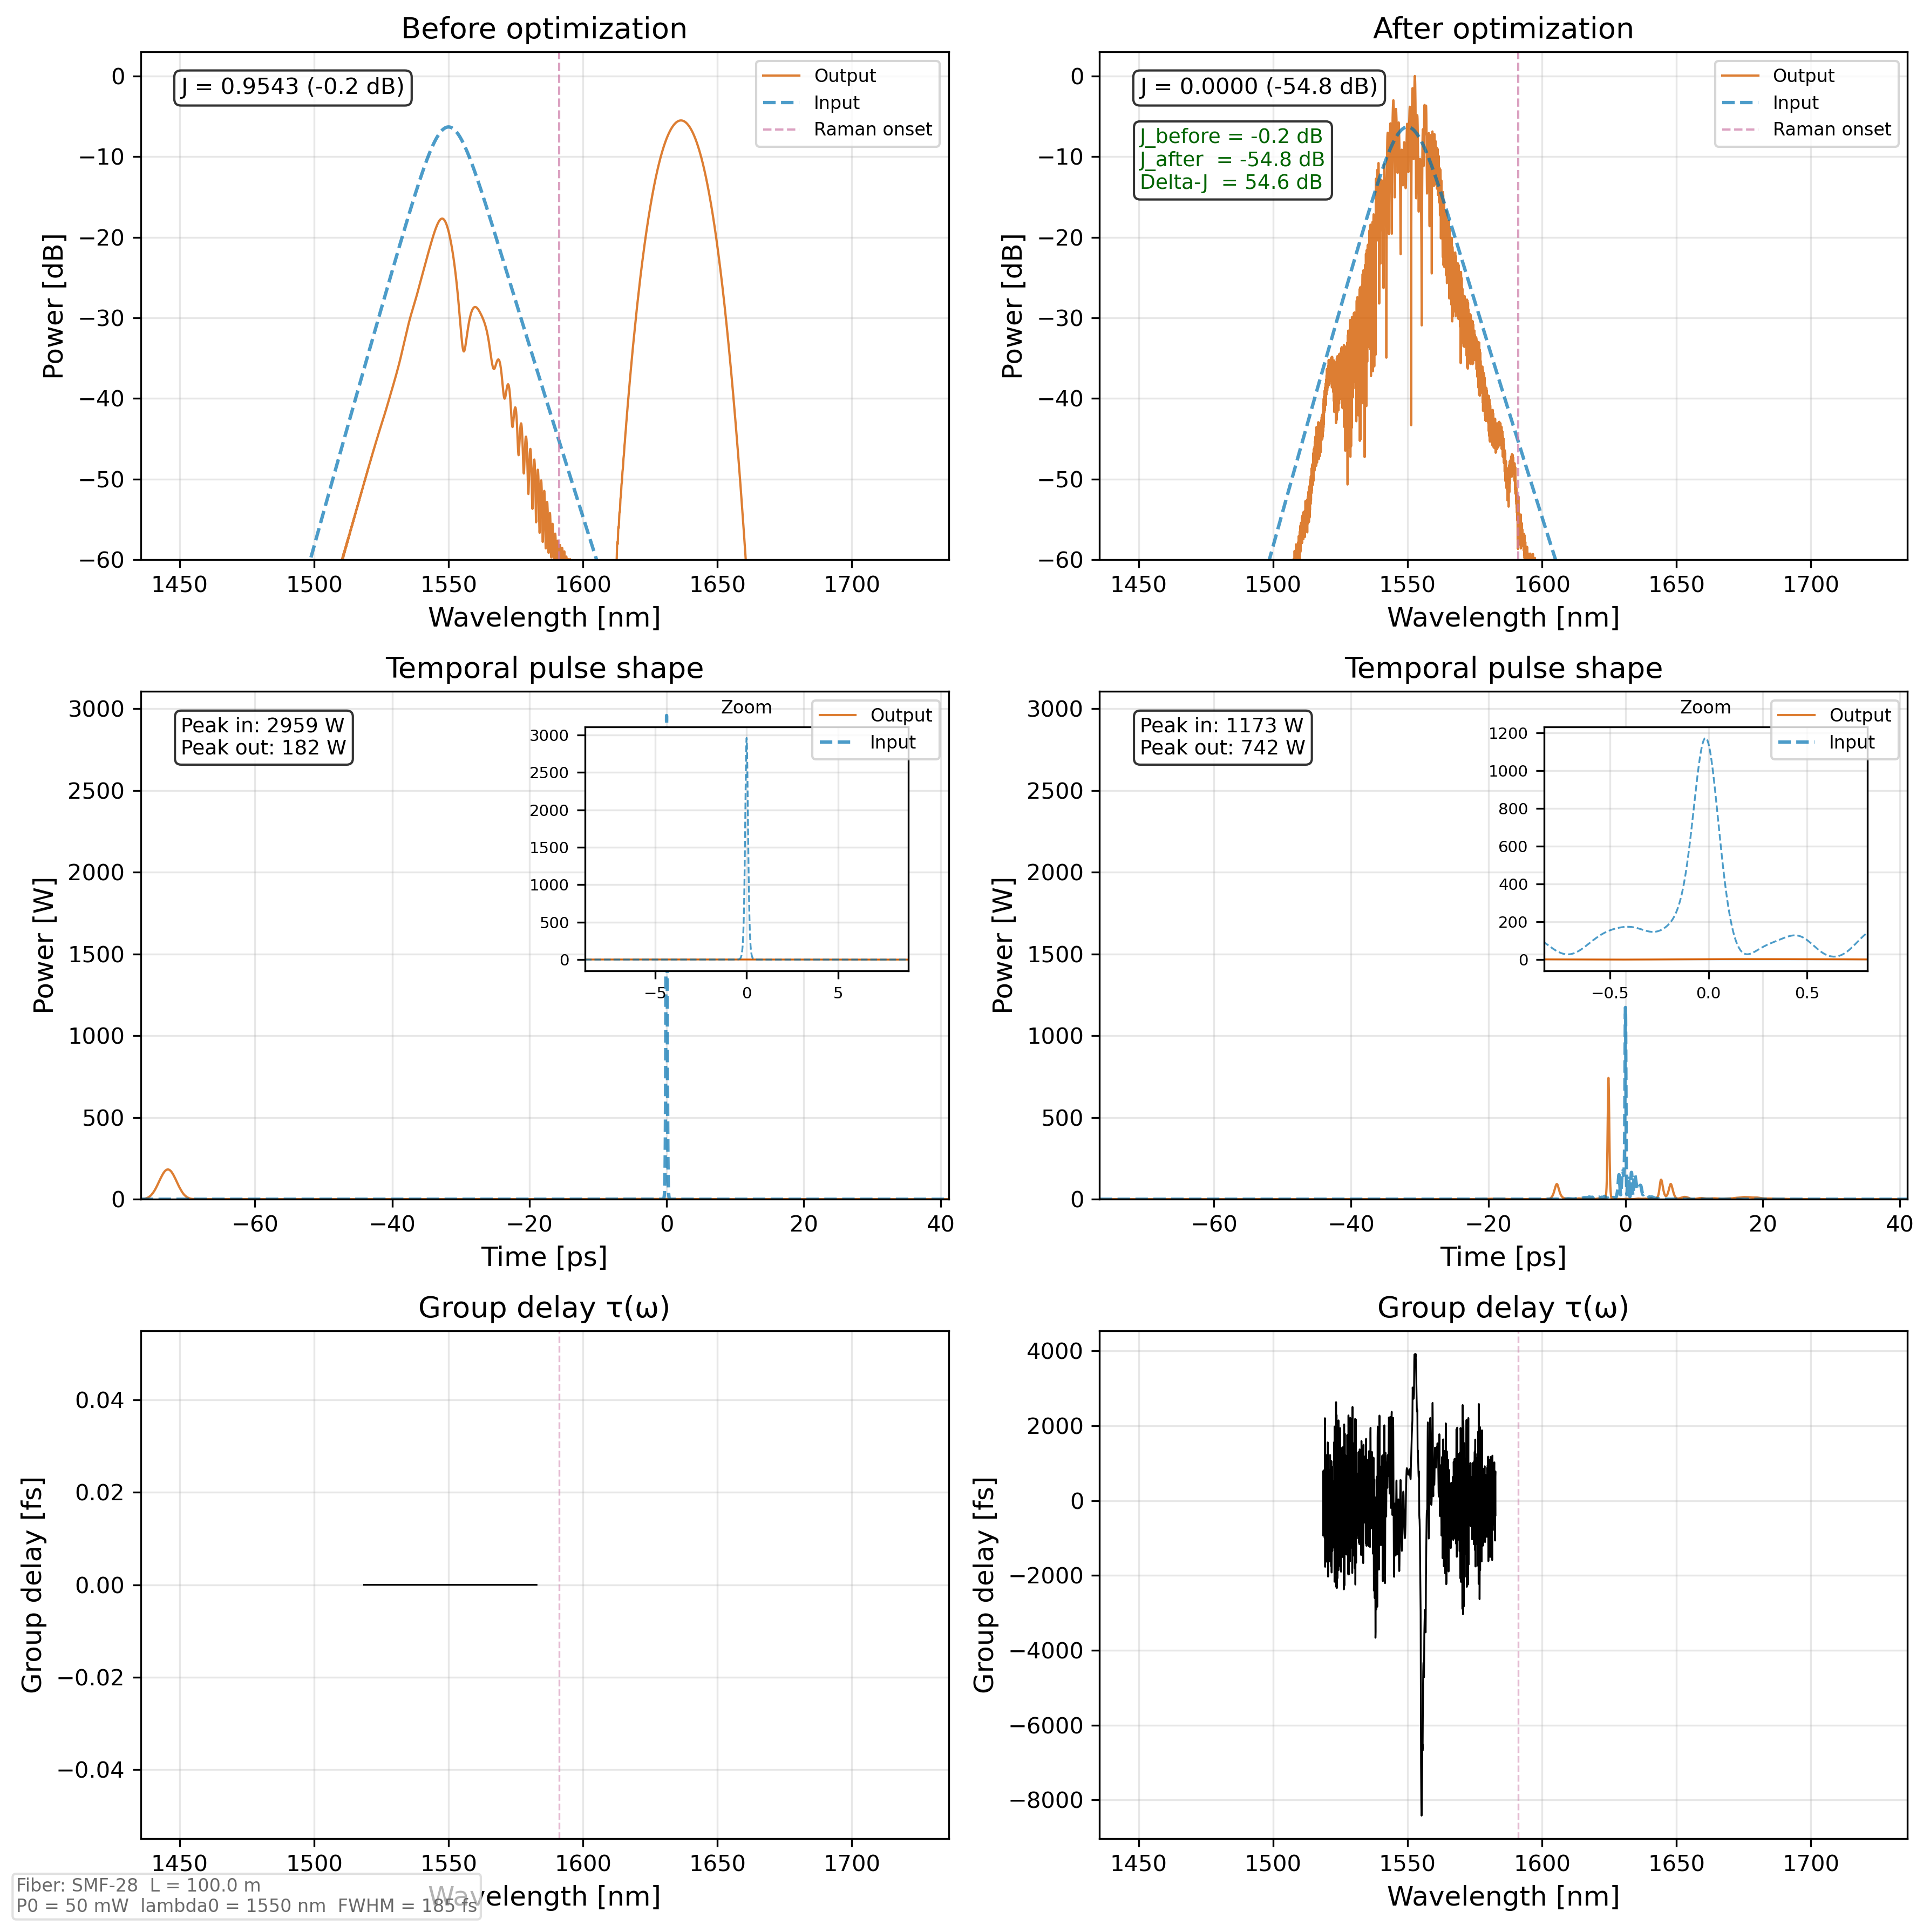
\includegraphics[width=0.82\textwidth]{phase21_100m_phase_profile.png}
\end{center}
\emph{Phase 21 honest-grid reproduction of Session~F's 100~m
warm-start optimum: $J = -54.77$~dB, BC edge $8.47\times10^{-6}$,
$\Delta E / E \le 4.91\times10^{-4}$. Four-panel standard image set
(input/output spectrum, wrapped/unwrapped phase, group delay). This
is the lower-bound anchor for the 100~m discussion; the overlay
below shows how a pure quadratic reproduces the suppression.}

\begin{center}
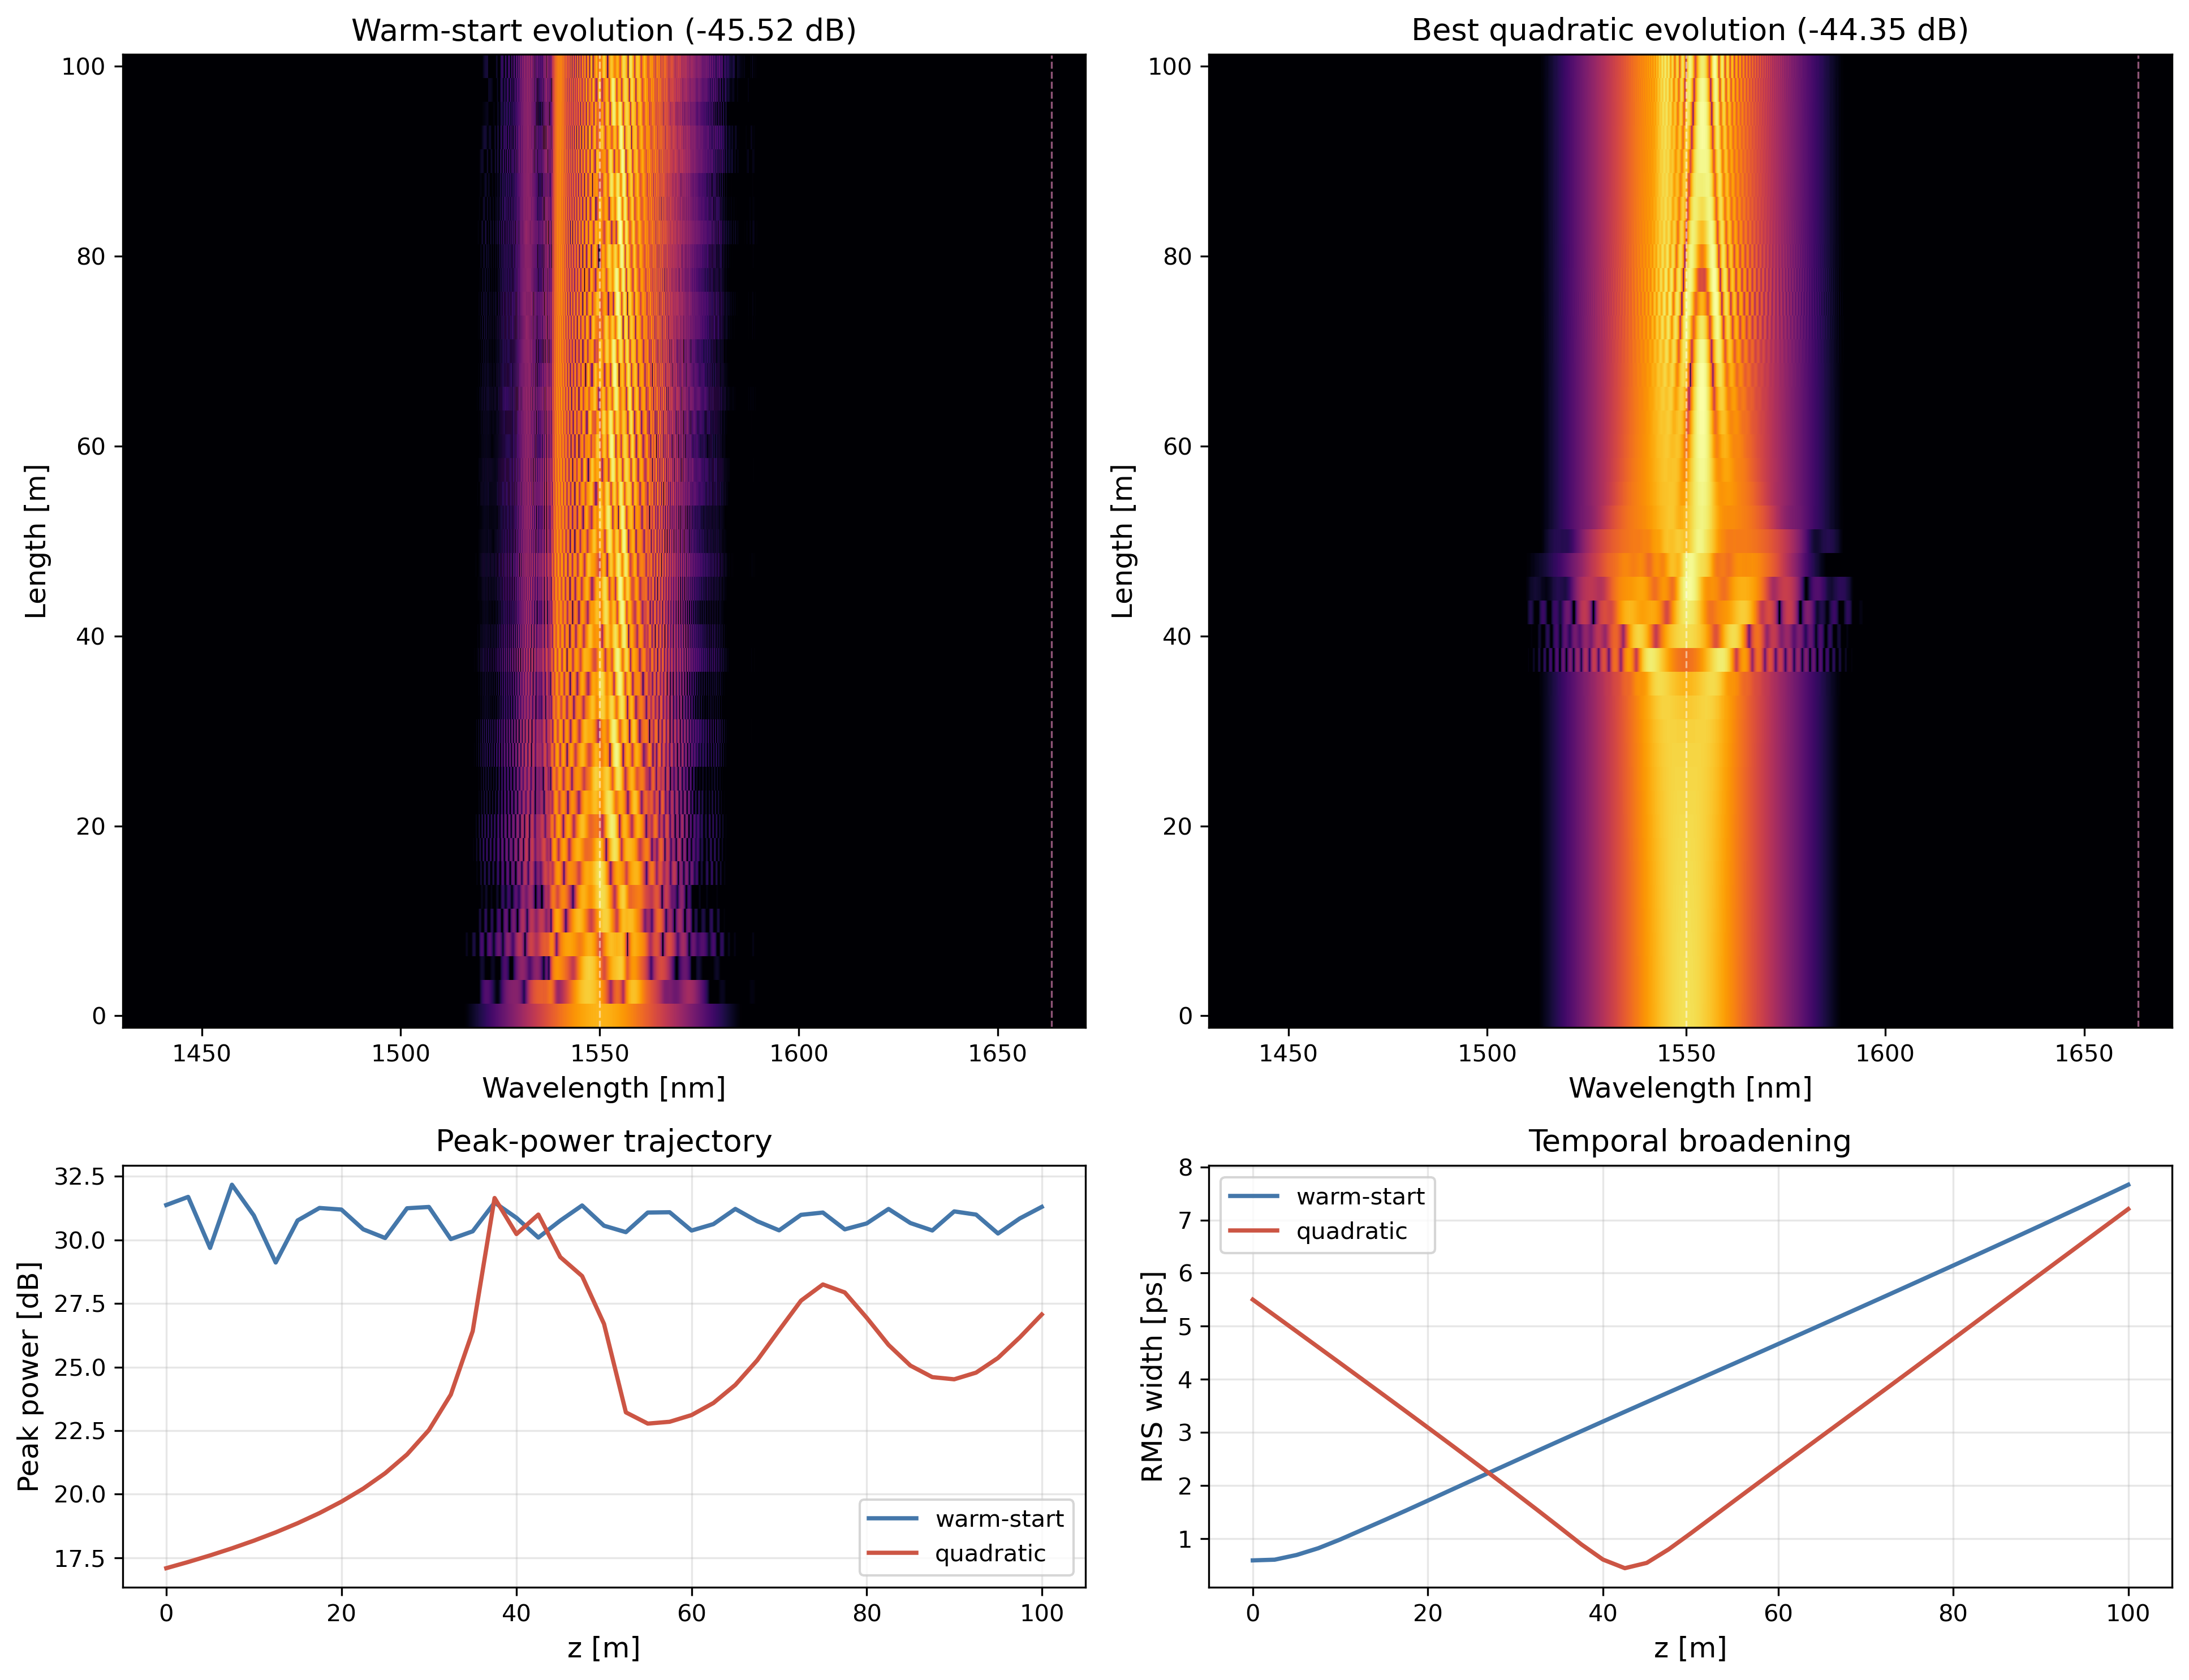
\includegraphics[width=0.92\textwidth]{phase23_warm_vs_gdd_p1_overlay.png}
\end{center}
\emph{Warm-start $\varphi_\text{opt}$@2m (blue) vs the matched
$\text{GDD}{=}+1$~ps$^2$ quadratic chirp (orange) at 100~m. The
trajectory is visually similar and the endpoint suppression is within
$1.17$~dB: the 100~m transferability is accounted for by the
quadratic component.}

Weighted quadratic fit (by analytic sech$^2$ amplitude over the $\pm 5$~THz
signal band) to $\varphi_\text{opt}(\omega)$ yields $R^2 = 0.015$ at 100~m
and $R^2 = 0.037$ at 2~m --- the optimal phase is \textbf{not a low-order
polynomial chirp}: $\lesssim$4\% of the bandwidth-weighted variance is
captured by a quadratic. This \emph{non-polynomial} finding is
independently defensible from the Phase 23 matched-quadratic result: at
100~m the endpoint $J$ is reached by generic pre-chirp, but
$\varphi_\text{opt}(\omega)$ itself is not a polynomial approximation
of that pre-chirp on the signal band --- the non-quadratic residual
structure does not change the endpoint depth but does characterise
what L-BFGS is parameterising. The physics thread worth following is
this non-polynomial residual, not the $a_2$-scaling reading below.

\textbf{Caveat (time window).} At 100~m the Stokes-band walk-off
$|\beta_2|\,L\,\Delta\omega_R \approx 177$~ps exceeds the 160~ps window,
so the \emph{flat}-phase reference ($J_\text{flat} = -0.20$~dB,
BC~$=0.68$, $\Delta E/E = 4.85\times10^{-2}$) has Stokes energy walking
outside the window and being absorbed by the super-Gaussian attenuator.
The flat reference is therefore a biased lower bound on suppression; the
shaped cases are unaffected because they don't generate much Stokes. Future
re-run at $T=320$~ps would remove the bias. Artefact:
\texttt{results/raman/phase16/FINDINGS.md}.

\textbf{Not claimed:} an earlier draft reported $a_2(100\text{\,m}) /
a_2(2\text{\,m}) = -3.30$ compared to a pure-GVD prediction of $+50$. That
claim is \emph{withdrawn.} With $R^2 < 0.04$ the quadratic coefficient $a_2$
is not a physically meaningful descriptor of $\varphi_\text{opt}$, and the
absolute $|a_2|$ is 2--4 orders of magnitude below what pure-GVD
pre-compensation ($a_2 = -\beta_2 L/2$) would predict at either length. The
defensible finding is the non-polynomial one above, not the $a_2$-ratio
framing. Standard images:
\texttt{.planning/phases/21-numerical-recovery/images/phase21\_sessionf\_100m\_*\_phase\_profile.png};
\texttt{.planning/phases/23-matched-baseline/images/phase23\_warm\_vs\_\{gdd\_p1,matched\}\_overlay.png}.
\end{advisory}

\begin{flagged}
\textbf{Issue 2: Attenuator not in adjoint (minor).} The super-Gaussian temporal attenuator (\texttt{simulate\_disp\_mmf.jl}, line~34) modifies the field during forward propagation but is not accounted for in the adjoint equation. This creates a gradient inconsistency proportional to the attenuator's effect on the pulse. When the pulse stays within $85\%$ of the time window (as ensured by the boundary penalty), the attenuator is $\approx 1$ and the error is negligible ($< 10^{-6}$).
\end{flagged}

\begin{flagged}
\textbf{Issue 3: Penalty discussion needs scope clarification.} Earlier revisions of this document described the \emph{phase-only} Raman optimizer as if it implemented a broader family of smoothness / Tikhonov / TOD-style penalties. In the current codebase, the single-mode phase-only path in \texttt{scripts/raman\_optimization.jl} implements only:
\begin{itemize}
\item GDD penalty: $J_{\text{GDD}} = \lambda_{\text{GDD}} \sum_i (d^2\varphi/d\omega^2)_i^2 \cdot \Delta\omega$
\item Boundary penalty: $J_{\text{boundary}} = \lambda_b \cdot E_{\text{edges}}/E_{\text{total,input}}$
\end{itemize}
Other regularizers \emph{do} exist elsewhere in the repo --- for example the amplitude-only and multivariable paths implement Tikhonov / TV / flatness penalties on amplitude-like controls --- but those are different optimizers, not part of the core phase-only formulation being verified in this section. TOD appears in this project as a \emph{diagnostic chirp sweep} and polynomial decomposition basis, not as a production penalty term in the phase-only cost. The discrepancy is therefore a documentation-scope bug, not a missing-code bug.
\end{flagged}

\subsection{Correct but Could Be Improved}

\begin{enumerate}[leftmargin=*]
\item \textbf{ODE solver choices (Task 9):} Both forward and adjoint now use Tsit5 (order 5/4, $\texttt{reltol}=10^{-8}$). The adjoint was previously Vern9/$10^{-10}$ but was changed because the adjoint accuracy is bounded by Tsit5's 4th-order dense interpolant for the forward field, making higher-order adjoint solvers unnecessary. Taylor remainder slopes remain 2.00/2.04 with the matched solvers.

\item \textbf{GDD penalty may over-constrain (R5):} Penalizing $d^2\varphi/d\omega^2$ (group delay dispersion) directly suppresses the most natural physical mechanism for Raman control: pre-chirping the pulse to lower its peak power during propagation. The auto-tuning logic (line~338--344) attempts to balance this by setting $\lambda_{\text{GDD}}$ based on a ``physics-based GDD maximum,'' but this maximum is estimated from the pulse duration, not from an analysis of optimal chirp for Raman suppression. \textbf{Recommendation:} Run the optimization with $\lambda_{\text{GDD}} = 0$ to see how much suppression is achievable without regularization, then gradually increase $\lambda_{\text{GDD}}$ to trade smoothness for performance.

\item \textbf{Boundary penalty on input only:} The boundary penalty checks the \emph{input} pulse (after phase shaping) but not the \emph{output} pulse. If the optimization adds large GDD, the input pulse stretches in time. But the output pulse may stretch even more due to fiber dispersion. The \texttt{run\_optimization} function does check the output boundary post-hoc (line~376), but this check does not feed back into the optimization. \textbf{Recommendation:} Consider adding an output boundary penalty, though this would require propagating its gradient through the entire forward-adjoint pipeline (significantly more complex).
\end{enumerate}

\subsection{Is the Research Approach Sound? (R2, R3, R4)}

\textbf{R2 --- Is adjoint optimization established?} Yes. Adjoint-based gradient computation through nonlinear PDEs is a mature technique in fluid dynamics (dating to the 1970s), aerodynamic shape optimization, and seismic inversion. Its application to the NLSE specifically was demonstrated by Ganapathysubramanian and Zabaras (Optics Letters, 2019). The present implementation is a straightforward application of established methodology.

\textbf{R3 --- Are there better alternatives?} Spectral phase shaping is one of several approaches:
\begin{itemize}[leftmargin=*]
\item \textbf{Amplitude shaping:} Also implemented in this codebase (\texttt{amplitude\_optimization.jl}). Can reduce peak power directly but changes the input spectrum, which may be undesirable.
\item \textbf{Fiber design:} Large mode area fibers, photonic crystal fibers, or fibers with modified Raman gain spectra. More permanent but less flexible than pulse shaping.
\item \textbf{Shorter fibers / lower power:} Trivially effective but may conflict with other experimental requirements.
\item \textbf{Spectral filtering:} Post-propagation removal of Raman energy via gratings or filters. Does not prevent the energy transfer, just removes the result.
\end{itemize}

Phase shaping is attractive because it is \emph{non-invasive} (no fiber modification), \emph{energy-neutral} (same input pulse energy), and \emph{reconfigurable} (SLM can be reprogrammed). The main limitation is \textbf{realizability}: can the optimized phase profile $\varphi(\omega)$ actually be implemented with available SLM resolution and bandwidth?

\textbf{R4 --- Is the problem well-posed?} The cost function $J = E_{\text{band}}/E_{\text{total}}$ is bounded, differentiable, and has a global minimum at $J=0$ (which may or may not be achievable). The main concerns are:
\begin{itemize}[leftmargin=*]
\item \textbf{Local minima:} The GNLSE is highly nonlinear, and the cost landscape likely has multiple local minima. The multi-start test shows 1.52~dB spread, suggesting some landscape structure. More extensive multi-start studies are needed.
\item \textbf{Cheat solutions:} Could the optimizer find a phase that spreads energy outside the simulation window? The boundary penalty guards against this, but its effectiveness depends on $\lambda_b$.
\item \textbf{Realizability:} Rapidly oscillating $\varphi(\omega)$ may not be implementable. The GDD penalty partially addresses this, but a more direct constraint on the phase bandwidth would be better.
\end{itemize}

\begin{advisory}
\textbf{Fundamental limitation:} For sufficiently long fibers or high powers (soliton number $N \gg 1$), the Raman self-frequency shift is a robust consequence of the soliton dynamics and may not be suppressible by any input phase profile. The soliton adjusts its parameters during propagation, and the Raman shift depends on the \emph{instantaneous} pulse shape at each $z$, not just the input. For moderate parameters ($N \sim 2$--$5$, $L \sim 1$--$5$~m), phase shaping has the best chance of working. For extreme parameters ($N > 10$), alternative approaches are likely needed.
\end{advisory}


% ═════════════════════════════════════════════════════════════════════════
\section{Code-to-Formulation Consistency Table}
\label{sec:consistency}

{\small
\begin{longtable}{p{1.6cm}p{3.5cm}p{3.5cm}p{0.7cm}p{3.5cm}}
\toprule
\textbf{Eq.\ \#} & \textbf{Claimed Location} & \textbf{Actual Location} & \textbf{OK?} & \textbf{Notes} \\
\midrule
\endhead

(1.2) & helpers.jl:187 & helpers.jl:187 & Y & Dispersion operator $D(\omega)$ \\

(1.3) & simulate\_disp\_mmf.jl:39--43 & simulate\_disp\_mmf.jl:39--43 & Y & Kerr: $\gamma|u|^2 u$ via Tullio \\

(1.4) & simulate\_disp\_mmf.jl:46--54 & simulate\_disp\_mmf.jl:46--54 & Y & Raman convolution via FFT \\

(1.5) & simulate\_disp\_mmf.jl:59 & simulate\_disp\_mmf.jl:59 & Y & Self-steepening $\omega/\omega_0$ \\

(1.6) & simulate\_disp\_mmf.jl:25--61 & simulate\_disp\_mmf.jl:25--61 & Y & Complete forward RHS \\

(2.1) & raman\_optimization.jl:62--64 & raman\_optimization.jl:62--64 & Y & Phase mask $u_0 = u_{00}e^{i\varphi}$ \\

(2.2) & common.jl:266--268 & common.jl:266--268 & Y & Cost function in \texttt{spectral\_band\_cost} \\

(2.3) & common.jl:269 & common.jl:269 & Y & Terminal condition $dJ$ \\

(3.2) & sensitivity\_disp\_mmf.jl:78 & sensitivity\_disp\_mmf.jl:78 & Y & Four adjoint terms \\

(3.3) T1 & sensitivity\_disp\_mmf.jl:130 & sensitivity\_disp\_mmf.jl:130--133 & Y & Term 1: $\lambda\cdot\partial f_{KR1}^*/\partial u^*$ \\

(3.3) T2 & sensitivity\_disp\_mmf.jl:142 & sensitivity\_disp\_mmf.jl:142--145 & Y & Term 2: $(1-f_R)\lambda^*\cdot\partial f_K/\partial u^*$ \\

(3.3) T3 & sensitivity\_disp\_mmf.jl:93 & sensitivity\_disp\_mmf.jl:93--100 & Y & Term 3: Raman conjugate \\

(3.3) T4 & sensitivity\_disp\_mmf.jl:112 & sensitivity\_disp\_mmf.jl:112--120 & Y & Term 4: Raman direct \\

(3.4) & sensitivity\_disp\_mmf.jl:296 & sensitivity\_disp\_mmf.jl:296 & Y & IP terminal condition \\

(4.2) & raman\_optimization.jl:91 & raman\_optimization.jl:91 & Y & Gradient formula \\

(5.1) & Julia FFT docs & --- & Y & FFT conventions documented \\

(5.3) & helpers.jl:181--183 & helpers.jl:181--183 & Y & Raman discretization (with overflow fix) \\

(5.4) & helpers.jl / common.jl & various & Y & Initial sech$^2$ pulse \\

\bottomrule

\caption{Equation-to-code consistency for the \texttt{smf-gain-noise/} repository (v2, 2026-03-26). All line numbers reverified against current codebase. All formulas are mathematically correct.}
\end{longtable}
}


% ═════════════════════════════════════════════════════════════════════════
\section{Regularization Analysis (R5, Task 12)}
\label{sec:regularization}

\subsection{GDD Penalty}

\textbf{Mathematical form:}
\begin{equation}
J_{\text{GDD}} = \lambda_{\text{GDD}} \sum_{i=2}^{N_t-1} \frac{(\varphi_{i+1} - 2\varphi_i + \varphi_{i-1})^2}{\Delta\omega^3}
\label{eq:gdd_penalty}
\end{equation}

This approximates the continuous functional $\lambda_{\text{GDD}}\int (d^2\varphi/d\omega^2)^2\,d\omega$ using the standard 3-point stencil for the second derivative: $(d^2\varphi/d\omega^2)_i \approx (\varphi_{i+1} - 2\varphi_i + \varphi_{i-1})/\Delta\omega^2$. Squaring and multiplying by $\Delta\omega$ for the integral gives the $\Delta\omega^{-3}$ normalization.

\textbf{Gradient derivation:} Let $d_i = \varphi_{i+1} - 2\varphi_i + \varphi_{i-1}$. Then:
\begin{equation}
\pdv{J_{\text{GDD}}}{\varphi_k} = \frac{2\lambda_{\text{GDD}}}{\Delta\omega^3}\sum_i d_i \pdv{d_i}{\varphi_k}
\end{equation}
Since $\partial d_i/\partial\varphi_k = \delta_{k,i+1} - 2\delta_{k,i} + \delta_{k,i-1}$, summing over $i$:
\begin{equation}
\pdv{J_{\text{GDD}}}{\varphi_k} = \frac{2\lambda_{\text{GDD}}}{\Delta\omega^3}(d_{k-1} - 2d_k + d_{k+1})
\end{equation}

The code (\texttt{raman\_optimization.jl}, lines 97--112) accumulates the gradient by looping over $i$ and distributing each $d_i$'s contribution to its three neighbors:
\begin{lstlisting}
coeff = 2 * l_gdd * inv_Dw3 * d2
grad_total[i-1, m] += coeff
grad_total[i, m]   -= 2 * coeff
grad_total[i+1, m] += coeff
\end{lstlisting}

After accumulation over all $i$, \texttt{grad\_total[k]} $= (2\lambda_{\text{GDD}}/\Delta\omega^3)(d_{k-1} - 2d_k + d_{k+1})$.

\begin{verified}
The GDD penalty and its gradient are correctly implemented. The $\Delta\omega^{-3}$ normalization is the correct factor for grid-independent discretization of $\int(d^2\varphi/d\omega^2)^2\,d\omega$.
\end{verified}

\subsection{Boundary Penalty}

\textbf{Mathematical form:}
\begin{equation}
J_b = \lambda_b \frac{E_{\text{edges}}}{E_{\text{total,in}}} = \lambda_b \frac{\sum_n m_n |u_t^{(0)}[n]|^2}{\sum_n |u_t^{(0)}[n]|^2}
\end{equation}
where $m_n$ is the edge mask (1 for the first and last 5\% of the time grid, 0 elsewhere), and $u_t^{(0)} = \IFFT(u_{\omega,0}^{\text{shaped}})$ is the input pulse in the time domain.

\textbf{Gradient derivation:} Since $u_{\omega,0}^{\text{shaped}} = u_{\omega,00}e^{i\varphi}$ and $u_t^{(0)} = \IFFT(u_{\omega,0}^{\text{shaped}})$:
\begin{align}
\pdv{J_b}{\varphi_k} &= \frac{\lambda_b}{E_{\text{total,in}}} \cdot 2\Real\!\sum_n m_n\, u_t^{(0)*}[n]\,\pdv{u_t^{(0)}[n]}{\varphi_k}
\end{align}

Using Julia's IFFT convention ($\IFFT(x)_n = \frac{1}{N}\sum_k x_k e^{2\pi ikn/N}$):
\begin{equation}
\pdv{u_t^{(0)}[n]}{\varphi_k} = \frac{i}{N} u_{\omega,0}^{\text{shaped}}[k]\, e^{2\pi ikn/N}
\end{equation}

Substituting and simplifying:
\begin{equation}
\pdv{J_b}{\varphi_k} = \frac{2\lambda_b}{N\,E_{\text{total,in}}} \Imag\!\left[\overline{u_{\omega,0}^{\text{shaped}}[k]} \cdot \FFT(m \cdot u_t^{(0)})[k]\right]
\end{equation}

\begin{verified}
Code (\texttt{raman\_optimization.jl}, line~134):
\begin{lstlisting}
coeff = 2 * l_boundary / (Nt_b * E_total_input)
grad_boundary_w = coeff .* imag.(conj.(uw0_shaped) .* fft(mask_edge .* ut0, 1))
\end{lstlisting}
This exactly matches the derived gradient. The $1/N_t$ factor comes from the adjoint of IFFT being $(1/N)\cdot$FFT. \textbf{Correct.}
\end{verified}

\subsection{Assessment of Regularization Choices}

\begin{enumerate}[leftmargin=*]
\item \textbf{Is the GDD penalty standard?} Penalizing the second derivative of the phase (a Sobolev $H^2$ semi-norm) is standard in spectral phase retrieval and pulse compression. It is commonly used in pulse shaping to enforce smoothness. In PDE-constrained optimization, similar ``Tikhonov-type'' penalties on control derivatives are standard (Hinze et al., 2009).

\item \textbf{Could GDD penalty prevent finding good solutions?} Yes, if the optimal Raman suppression strategy involves significant pre-chirping. The auto-tuned $\lambda_{\text{GDD}}$ uses a maximum GDD estimated from the pulse duration, which may be too conservative. Running without GDD penalty would reveal whether the optimizer exploits chirp as a suppression mechanism.

\item \textbf{Is the boundary penalty on the right signal?} Penalizing the input pulse is necessary because the optimization \emph{controls} the input. If the input pulse is too broad, the output will be even broader. However, checking only the input misses cases where nonlinear propagation broadens the pulse beyond the window. The post-hoc output check partially addresses this.
\end{enumerate}


% ═════════════════════════════════════════════════════════════════════════
% APPENDICES
% ═════════════════════════════════════════════════════════════════════════

\appendix

\section{Notation Table}
\label{app:notation}

{\small
\begin{longtable}{p{2.5cm}p{6cm}p{2.5cm}p{2cm}}
\toprule
\textbf{Symbol} & \textbf{Meaning} & \textbf{Units} & \textbf{First Use} \\
\midrule
\endhead

$u(z,t)$ & Complex field envelope & $\sqrt{\text{W}}$ & Eq.~(1) \\
$\hat{u}_\omega$ & Frequency-domain field (lab frame) & $\sqrt{\text{W}}\cdot$ps & Eq.~(1) \\
$\tilde{u}_\omega$ & Interaction picture field & $\sqrt{\text{W}}\cdot$ps & Eq.~(2) \\
$D(\omega)$ & Dispersion operator & m$^{-1}$ & Eq.~(1) \\
$\beta_n$ & $n$-th dispersion coefficient & s$^n$/m & Sec.~2.1 \\
$\gamma$ & Nonlinear coefficient & W$^{-1}$m$^{-1}$ & Eq.~(1) \\
$f_R$ & Raman fraction & --- & Eq.~(1) \\
$h_R(t)$ & Raman response function & ps$^{-1}$ & Eq.~(4) \\
$\tau_1, \tau_2$ & Raman time constants & fs & Eq.~(4) \\
$\hat{S}(\omega)$ & Self-steepening operator & --- & Eq.~(1) \\
$\omega_0$ & Carrier angular frequency & rad/ps & Eq.~(1) \\
$\varphi(\omega)$ & Spectral phase (optimization variable) & rad & Eq.~(5) \\
$J$ & Cost function (Raman fraction) & --- & Eq.~(6) \\
$\lambda(z)$ & Adjoint (co-state) variable & varies & Eq.~(8) \\
$\mathcal{B}$ & Raman frequency band ($\Delta f < -5$~THz) & --- & Eq.~(6) \\
$N_t$ & Number of time/frequency samples & --- & Sec.~2 \\
$\Delta t$ & Time step & ps & Sec.~2 \\
$L$ & Fiber length & m & Sec.~2 \\
$L_D$ & Dispersion length & m & Sec.~2 \\
$L_{NL}$ & Nonlinear length & m & Sec.~2 \\
$N$ & Soliton number & --- & Sec.~2 \\

\bottomrule
\end{longtable}
}


\section{Complete Derivation Worksheets}
\label{app:derivations}

\subsection{Worksheet: Wirtinger Derivatives}

For a function $f(u, u^*)$ where $u = x + iy$ is complex, the Wirtinger derivatives are:
\begin{align}
\pdv{f}{u} &= \frac{1}{2}\left(\pdv{f}{x} - i\pdv{f}{y}\right) \\
\pdv{f}{u^*} &= \frac{1}{2}\left(\pdv{f}{x} + i\pdv{f}{y}\right)
\end{align}

\textbf{Key properties:}
\begin{enumerate}
\item $\partial(u \cdot u^*)/\partial u^* = u$
\item $\partial(u \cdot u^*)/\partial u = u^*$
\item For real $J(u,u^*)$: $(\partial J/\partial u)^* = \partial J/\partial u^*$
\item The total differential: $dJ = \sum_k (\partial J/\partial u_k)\,du_k + (\partial J/\partial u_k^*)\,du_k^*$
\end{enumerate}

\subsection{Worksheet: Terminal Condition Derivation}

\textbf{Given:} $J = E_b/E_t$ where $E_b = \sum_{\omega \in \mathcal{B}}|u_\omega|^2$, $E_t = \sum_\omega |u_\omega|^2$.

\textbf{Step 1:} $\partial|u_\omega|^2/\partial u_k^* = \partial(u_\omega u_\omega^*)/\partial u_k^* = u_\omega\,\delta_{\omega k}$

\textbf{Step 2:} $\partial E_b/\partial u_k^* = \mathbb{1}_\mathcal{B}(k)\cdot u_k$

\textbf{Step 3:} $\partial E_t/\partial u_k^* = u_k$

\textbf{Step 4:} Quotient rule: $\partial J/\partial u_k^* = (\partial E_b/\partial u_k^* \cdot E_t - E_b \cdot \partial E_t/\partial u_k^*)/E_t^2$
\begin{align}
&= \frac{\mathbb{1}_\mathcal{B}(k)\cdot u_k \cdot E_t - E_b \cdot u_k}{E_t^2} = \frac{u_k(\mathbb{1}_\mathcal{B}(k) - J)}{E_t} \quad\checkmark
\end{align}

\subsection{Worksheet: Chain Rule Through Phase Mask}

\textbf{Given:} $u_0(\omega) = u_{00}(\omega)e^{i\varphi(\omega)}$, $\delta J = 2\Real\sum_\omega \lambda_0^*\,\delta u_0$.

\textbf{Step 1:} $\delta u_0(\omega) = u_{00}(\omega)\cdot ie^{i\varphi(\omega)}\cdot\delta\varphi(\omega) = i\,u_0(\omega)\,\delta\varphi(\omega)$

\textbf{Step 2:} $\delta J = 2\Real\sum_\omega \lambda_0^*(\omega)\cdot i\,u_0(\omega)\cdot\delta\varphi(\omega)$

\textbf{Step 3:} Since $\delta\varphi$ is real and arbitrary: $\partial J/\partial\varphi(\omega) = 2\Real[\lambda_0^*(\omega)\cdot i\cdot u_0(\omega)]$

\textbf{Step 4:} Equivalently: $= -2\Imag[\lambda_0^*(\omega)\cdot u_0(\omega)]$ since $\Real(iz) = -\Imag(z)$.~$\checkmark$

\subsection{Worksheet: Interaction Picture Adjoint Transformation}

\textbf{Given:} Forward transformation $u = Mu_{\text{IP}}$ where $M = e^{iDz}$ (diagonal, $D$ real).

\textbf{Goal:} Find $\lambda_{\text{IP}}$ such that $\langle\lambda, \delta u\rangle = \langle\lambda_{\text{IP}}, \delta u_{\text{IP}}\rangle$.

\textbf{Step 1:} $\delta u = M\,\delta u_{\text{IP}}$ (linearize the transformation).

\textbf{Step 2:} $\langle\lambda, M\,\delta u_{\text{IP}}\rangle = \langle M^\dagger\lambda, \delta u_{\text{IP}}\rangle$ (definition of adjoint).

\textbf{Step 3:} $M^\dagger = (e^{iDz})^* = e^{-iDz}$ ($D$ is real diagonal).

\textbf{Step 4:} $\lambda_{\text{IP}} = e^{-iDz}\lambda$.~$\checkmark$

\subsection{Worksheet: GDD Penalty Gradient}

\textbf{Given:} $J_{\text{GDD}} = \alpha\sum_{i=2}^{N-1}d_i^2$ where $d_i = \varphi_{i+1}-2\varphi_i+\varphi_{i-1}$ and $\alpha = \lambda_{\text{GDD}}/\Delta\omega^3$.

\textbf{Step 1:} $\partial d_i/\partial\varphi_k = \delta_{k,i+1} - 2\delta_{k,i} + \delta_{k,i-1}$

\textbf{Step 2:} $\partial J/\partial\varphi_k = 2\alpha\sum_i d_i(\delta_{k,i+1} - 2\delta_{k,i} + \delta_{k,i-1})$

\textbf{Step 3:} The sum picks out three terms: $i=k-1$ (coefficient $+1$), $i=k$ (coefficient $-2$), $i=k+1$ (coefficient $+1$).

\textbf{Step 4:} $\partial J/\partial\varphi_k = 2\alpha(d_{k-1} - 2d_k + d_{k+1})$.~$\checkmark$

This is the discrete biharmonic operator applied to $\varphi$ --- the fourth finite-difference derivative.


\section{Code Audit Findings}
\label{app:code_audit}

\subsection{simulate\_disp\_mmf.jl (Forward Solver)}

\begin{center}
\begin{tabular}{p{1.5cm}p{4cm}p{3cm}p{1cm}}
\toprule
\textbf{Lines} & \textbf{Operation} & \textbf{Math} & \textbf{OK?} \\
\midrule
28--29 & Compute $e^{\pm iDz}$ & Interaction picture phases & Y \\
31 & $u_\omega = e^{iDz}\tilde{u}$ & Lab frame recovery & Y \\
33 & FFT of $u_\omega$ & $u_t = \FFT(u_\omega)$ & Y \\
34 & Apply attenuator & Non-physical window & $\star$ \\
35--36 & Extract Re, Im & $v = \Real(u_t)$, $w = \Imag(u_t)$ & Y \\
39--43 & Kerr $\eta_K$ & $(1-f_R)\gamma|u|^2 u$ & Y \\
46--54 & Raman $\eta_R$ & $\gamma(h_R*|u|^2)u$ via FFT & Y \\
57 & Sum NL terms & $\eta = \eta_K + \eta_R$ & Y \\
58 & IFFT of $\eta$ & To frequency domain & Y \\
59 & Self-steepening & $\times\omega/\omega_0$ & Y \\
60 & IP projection & $d\tilde{u}/dz = ie^{-iDz}\eta_\omega$ & Y \\
\bottomrule
\end{tabular}
\end{center}

$\star$ = Attenuator is functionally correct but not in the adjoint. See Issue~2.

\subsection{sensitivity\_disp\_mmf.jl (Adjoint Solver)}

\begin{center}
\begin{tabular}{p{1.5cm}p{4.5cm}p{2.5cm}p{1cm}}
\toprule
\textbf{Lines} & \textbf{Operation} & \textbf{Math} & \textbf{OK?} \\
\midrule
20--21 & Compute $e^{\pm iDz}$ & IP phases & Y \\
23--24 & $\lambda_\omega = e^{iDz}\tilde\lambda \cdot \tau_\omega$ & Lab frame + self-steep & Y \\
25--28 & FFT/conj of $\lambda$ & $\lambda_t$, $\lambda^*_\omega$ & Y \\
29--33 & Recover $u(z)$ from sol & Forward field at $z$ & Y \\
35 & \texttt{calc\_$\delta$s!} & $\delta_{K1}$, $\delta_{K2}$ from $u$ & Y \\
36--42 & Raman convolution & $h_R * \delta_{K1}$ & Y \\
44 & Term 1 & $\lambda\cdot\partial f_{KR1}^*/\partial u^*$ & Y \\
45 & Term 2 ($\times N_t$) & $(1-f_R)\lambda^*\cdot\partial f_K/\partial u^*$ & Y \\
46 & Term 3 ($\div N_t$) & Raman conjugate term & Y \\
47--48 & Term 4 ($\times N_t$) & Raman direct term & Y \\
50 & Sum all terms & $d\tilde\lambda/dz$ & Y \\
296 & Terminal cond.\ IP & $\tilde\lambda_L = e^{-iDL}\lambda_L$ & Y \\
301 & Backward ODE & $(L, 0)$, Tsit5, $10^{-8}$ & Y \\
\bottomrule
\end{tabular}
\end{center}

The $N_t$ factors in Terms 2, 3, 4 arise from the FFT/IFFT normalization asymmetry in Julia (\texttt{fft} unnormalized, \texttt{ifft} divides by $N$). Specifically:
\begin{itemize}[leftmargin=*]
\item The adjoint of \texttt{fft} (unnormalized forward) is $N_t \cdot$\texttt{ifft} (conjugate transpose of the DFT matrix).
\item The adjoint of \texttt{ifft} (normalized inverse) is $(1/N_t)\cdot$\texttt{fft}.
\end{itemize}
These factors are confirmed correct by the finite-difference gradient check.

\subsection{raman\_optimization.jl (Main Script)}

\begin{center}
\begin{tabular}{p{1.5cm}p{5cm}p{1cm}p{3cm}}
\toprule
\textbf{Lines} & \textbf{Function/Block} & \textbf{OK?} & \textbf{Notes} \\
\midrule
48--143 & \texttt{cost\_and\_gradient} & Y & Core pipeline correct \\
62--64 & Phase application & Y & \texttt{cis} = $e^{i\varphi}$ \\
74--77 & Lab frame output & Y & $u_L = e^{iDL}\tilde u_L$ \\
90 & Gradient formula & Y & $2\Real(\lambda_0^* \cdot iu_0)$ \\
97--112 & GDD penalty + gradient & Y & Verified derivation \\
114--137 & Boundary penalty + grad & Y & Verified derivation \\
179--198 & L-BFGS interface & Y & Log-scale cost with chain-rule-scaled gradient \\
212--243 & \texttt{validate\_gradient} & Y & Central FD, correct \\
272--302 & \texttt{chirp\_sensitivity} & Y & GDD/TOD sweeps correct \\
\bottomrule
\end{tabular}
\end{center}

$\star$ = Attenuator is functionally correct but not in the adjoint. See Issue~2.

\subsection{common.jl (Shared Functions)}

\begin{center}
\begin{tabular}{p{1.5cm}p{5cm}p{1cm}p{3cm}}
\toprule
\textbf{Lines} & \textbf{Function} & \textbf{OK?} & \textbf{Notes} \\
\midrule
253--269 & \texttt{spectral\_band\_cost} & Y & $J$ and $dJ$ correct \\
276--295 & \texttt{check\_boundary\_conditions} & Y & 5\% edge check \\
189--224 & \texttt{recommended\_time\_window} & Y & SPM-corrected (v2) \\
226--234 & \texttt{nt\_for\_window} & Y & Power-of-2 grid sizing (v2) \\
309--370 & \texttt{setup\_raman\_problem} & Y & Grid, fiber, pulse setup \\
361 & Band mask & Y & $\Delta f < -5$ THz (Stokes) \\
\bottomrule
\end{tabular}
\end{center}

\subsection{helpers.jl (Utilities)}

\begin{center}
\begin{tabular}{p{1.5cm}p{5cm}p{1cm}p{3cm}}
\toprule
\textbf{Lines} & \textbf{Function/Block} & \textbf{OK?} & \textbf{Notes} \\
\midrule
11--30 & \texttt{get\_disp\_sim\_params} & Y & Grid setup, attenuator \\
16 & Time array & Y & Centered: $[-T/2, T/2)$ \\
17 & Freq array & Y & fftshifted absolute freq \\
158--187 & \texttt{get\_disp\_fiber\_params\_user\_defined} & Y & Builds $D(\omega)$, $h_R$, $\gamma$ \\
176--177 & Raman response & Y & Blow--Wood, correct units \\
180 & $\beta$ vector & Y & $\beta_0=\beta_1=0$ (co-moving) \\
181 & Dispersion operator & Y & Correct polynomial + units \\
\bottomrule
\end{tabular}
\end{center}


% ═════════════════════════════════════════════════════════════════════════
\section{New Infrastructure (v2)}
\label{sec:new_infra}

The following additions were made after the initial verification and do not affect the core mathematical formulation. They are documented here for completeness.

\subsection{SPM-Corrected Time Window (Phase~7)}

The function \texttt{recommended\_time\_window()} (\texttt{common.jl}, line~191) computes a safe window from dispersive walk-off plus SPM-induced broadening:
\begin{align}
T_{\text{walk-off}} &= |\beta_2| \cdot L \cdot \Delta\omega_R \times 10^{12} \quad\text{[ps]} \\
\varphi_{NL} &= \gamma \cdot P_{\text{peak}} \cdot L \quad\text{[rad]} \\
\delta\omega_{\text{SPM}} &= 0.86 \cdot \varphi_{NL} / T_0 \quad\text{[rad/s, Agrawal Ch.~4 for sech$^2$]} \\
T_{\text{SPM}} &= |\beta_2| \cdot L \cdot \delta\omega_{\text{SPM}} \times 10^{12} \quad\text{[ps]} \\
T_{\text{window}} &= \max\!\left(5,\, \lceil \text{safety\_factor} \times (T_{\text{walk-off}} + T_{\text{SPM}} + 0.5) \rceil\right) \quad\text{[ps]}
\end{align}
where $\Delta\omega_R = 2\pi \times 13$~THz and $T_0 = \text{FWHM}/1.763$. The critical $0.86/T_0$ factor converts nonlinear phase (radians) to spectral broadening (rad/s) --- the v2 formula incorrectly used $\gamma P L$ directly as a frequency, which underestimated windows by 5--7$\times$ at high power.

\begin{advisory}
\textbf{v3: Auto-sizing.} \texttt{setup\_raman\_problem()} and \texttt{setup\_amplitude\_problem()} (common.jl, lines 348--359 and 427--438) now automatically override \texttt{time\_window} and \texttt{Nt} when the caller's values are smaller than \texttt{recommended\_time\_window()}. Previously only emitted a warning.
\end{advisory}

A companion function \texttt{nt\_for\_window()} (line~226) returns the smallest power-of-2 $N_t$ maintaining $\Delta t \leq 10.5$~fs temporal resolution.

\subsection{Parameter Sweep Infrastructure (Phase~7)}

\texttt{scripts/run\_sweep.jl} implements a systematic $L \times P$ grid sweep:
\begin{itemize}[leftmargin=*]
\item SMF-28: 4 lengths $\times$ 4 powers $= 16$ grid points
\item HNLF: 4 lengths $\times$ 4 (lower) powers $= 16$ grid points
\item 10-start robustness analysis on SMF-28 $L=2$~m, $P=0.30$~W
\end{itemize}

New visualization functions in \texttt{scripts/visualization.jl}:
\begin{itemize}[leftmargin=*]
\item \texttt{plot\_sweep\_heatmap()} --- $L \times P$ grid results as color map
\item \texttt{plot\_multistart\_histogram()} --- distribution of final costs across starts
\item \texttt{plot\_convergence\_overlay()} --- $J(\text{iteration})$ for all runs
\item \texttt{plot\_spectral\_overlay()} --- output spectra grouped by fiber type
\end{itemize}

These additions do not modify any core simulation, adjoint, or optimization code. The mathematical formulation and all previously verified equations remain unchanged.

\subsection{Log-Scale Cost Function (v3)}

The optimizer now defaults to minimizing $J_{\text{dB}} = 10\log_{10}(J)$ with gradient:
\begin{equation}
\pdv{J_{\text{dB}}}{\varphi} = \frac{10}{J\ln 10}\cdot\pdv{J}{\varphi}
\end{equation}

Code (\texttt{raman\_optimization.jl}, lines 97--107):
\begin{lstlisting}
if log_cost
    J_clamped = max(J, 1e-15)
    J_phys = 10.0 * log10(J_clamped)
    log_scale = 10.0 / (J_clamped * log(10.0))
    dJ_dphi_scaled = dJ_dphi .* log_scale
end
\end{lstlisting}

\begin{keyresult}
The log-scale cost improved suppression by 20--28~dB across all 24 sweep configurations, reaching $-78$~dB (SMF-28) and $-74$~dB (HNLF). Multi-start convergence improved from 0/10 to 10/10, with spread collapsing from 28.6~dB to 10.9~dB.
\end{keyresult}

\subsection{Boundary Verification (v3)}

Re-running 4 high-boundary-energy points with $2\times$ wider windows confirmed 3/4 \emph{improved} (optimizer uses extra room productively). One point lost 5.5~dB --- honest suppression $-66$~dB vs.\ reported $-71$~dB.

\subsection{Sweep Results}

\begin{figure}[H]
\centering
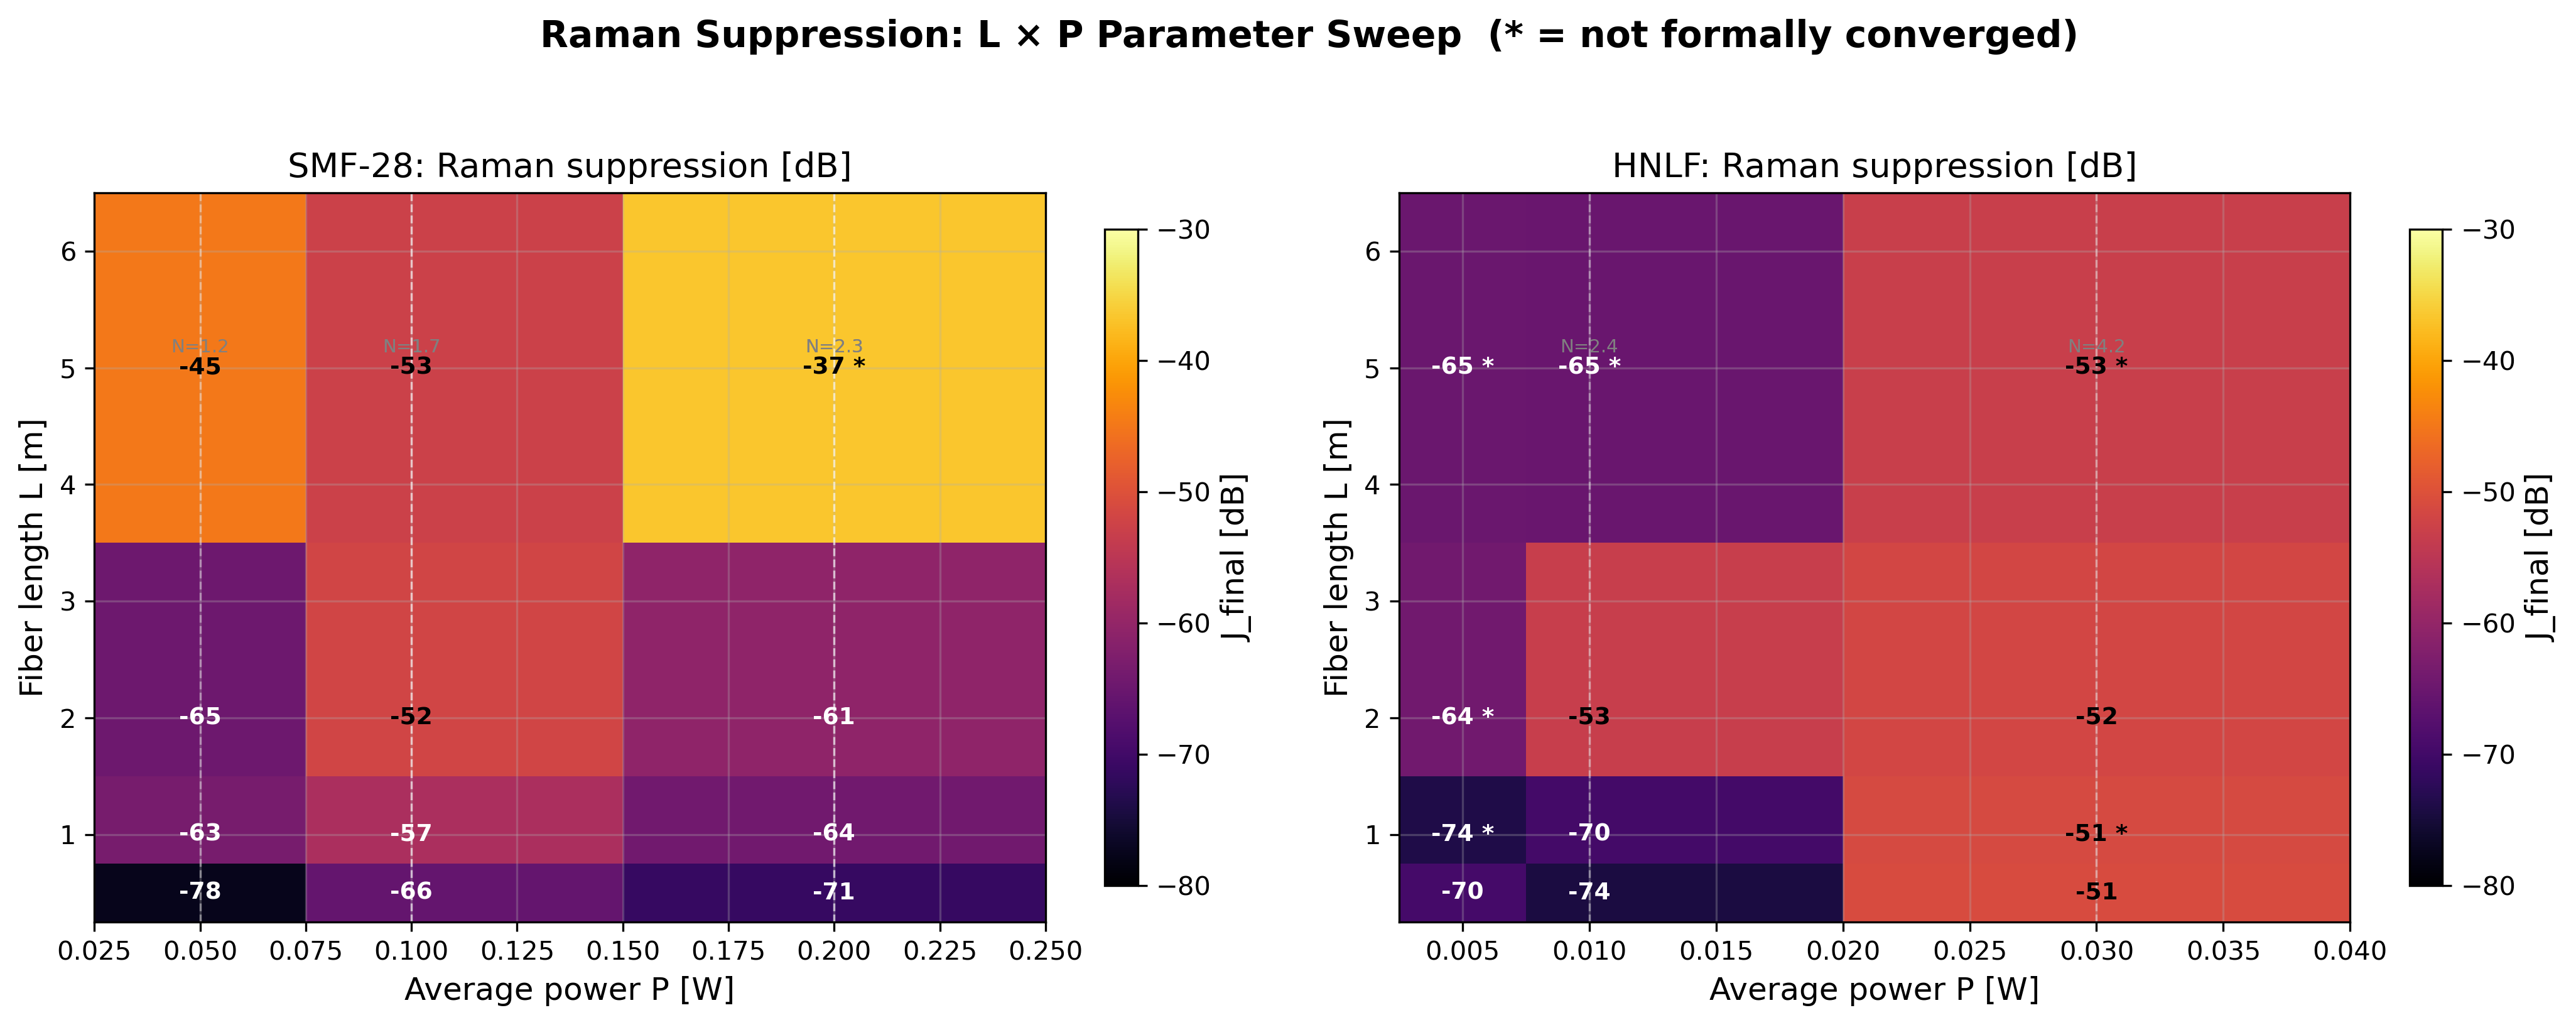
\includegraphics[width=\textwidth]{fig1_heatmaps.png}
\caption{Full parameter sweep: 24 configurations across SMF-28 and HNLF. Each cell annotated with $J_{\text{dB}}$; asterisk = not formally converged. All points achieve $> 36$~dB suppression.}
\label{fig:verification_heatmaps}
\end{figure}

\begin{figure}[H]
\centering
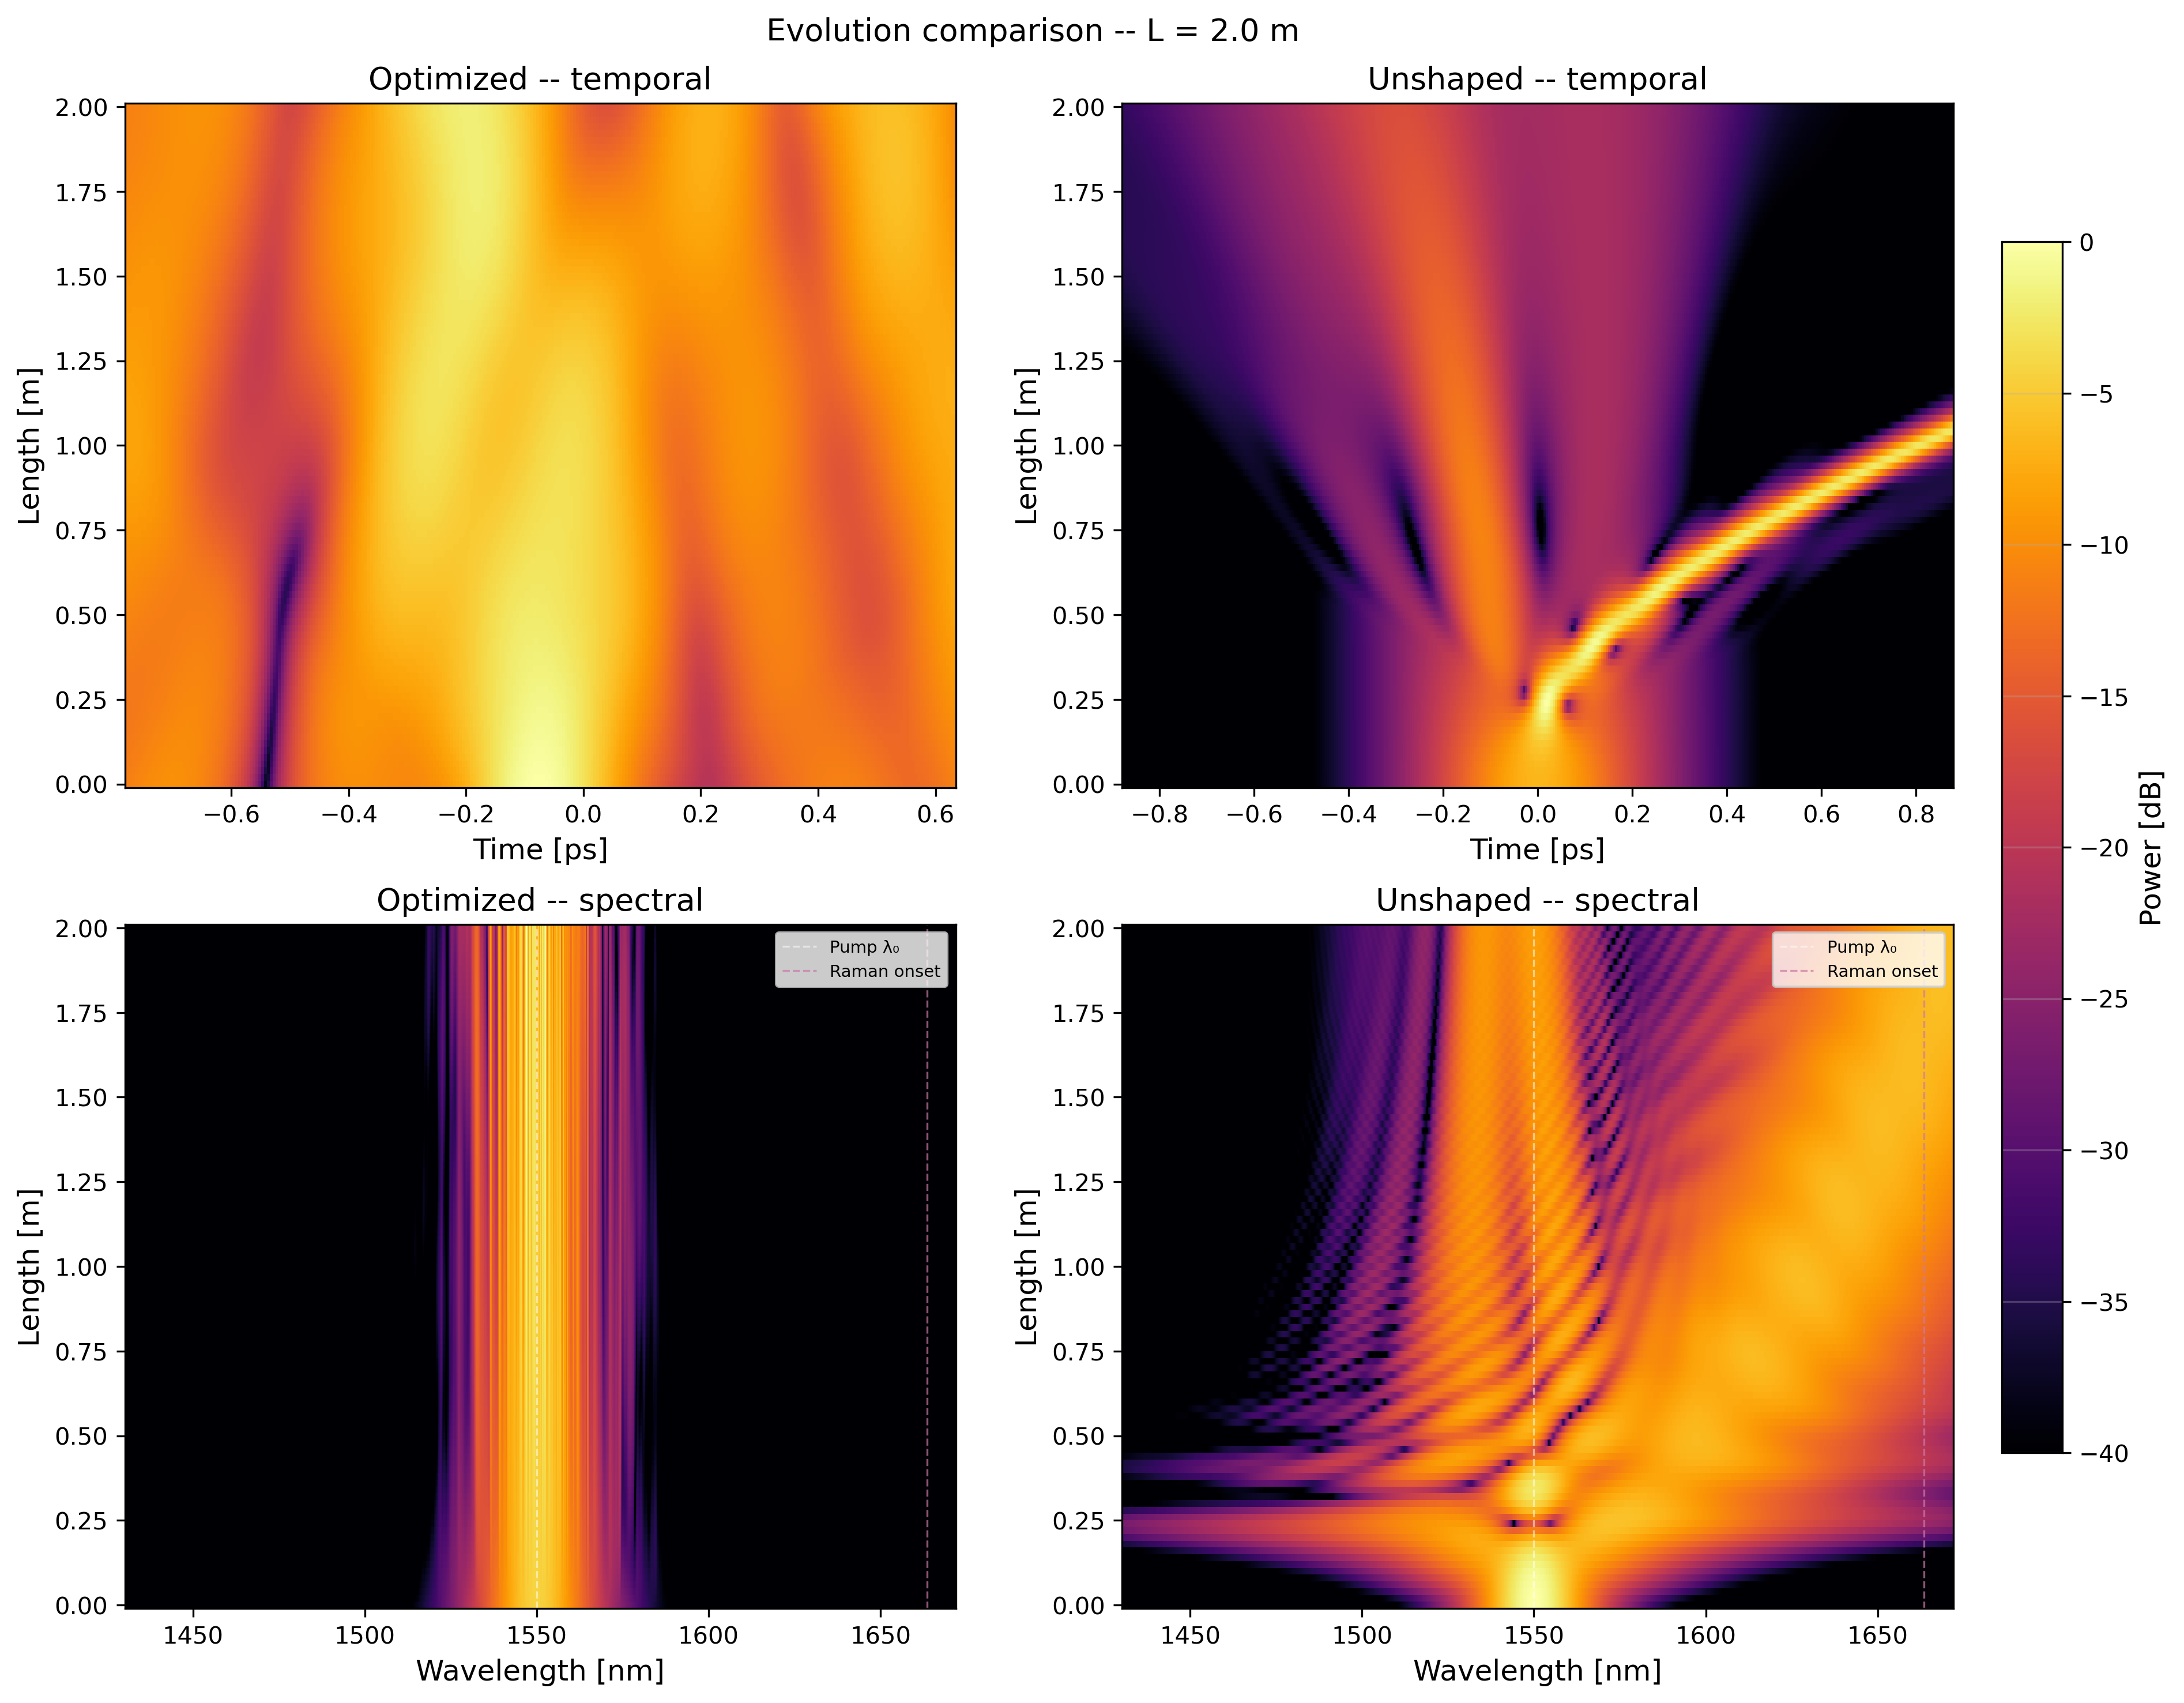
\includegraphics[width=\textwidth]{evolution_smf28_L2m_P02W.png}
\caption{Evolution comparison: SMF-28, L$=$2~m, P$=$0.20~W. Left: optimized --- spectrum stays confined. Right: unshaped --- soliton fission and Raman sidelobe visible past 1600~nm.}
\label{fig:verification_evolution}
\end{figure}

\begin{figure}[H]
\centering
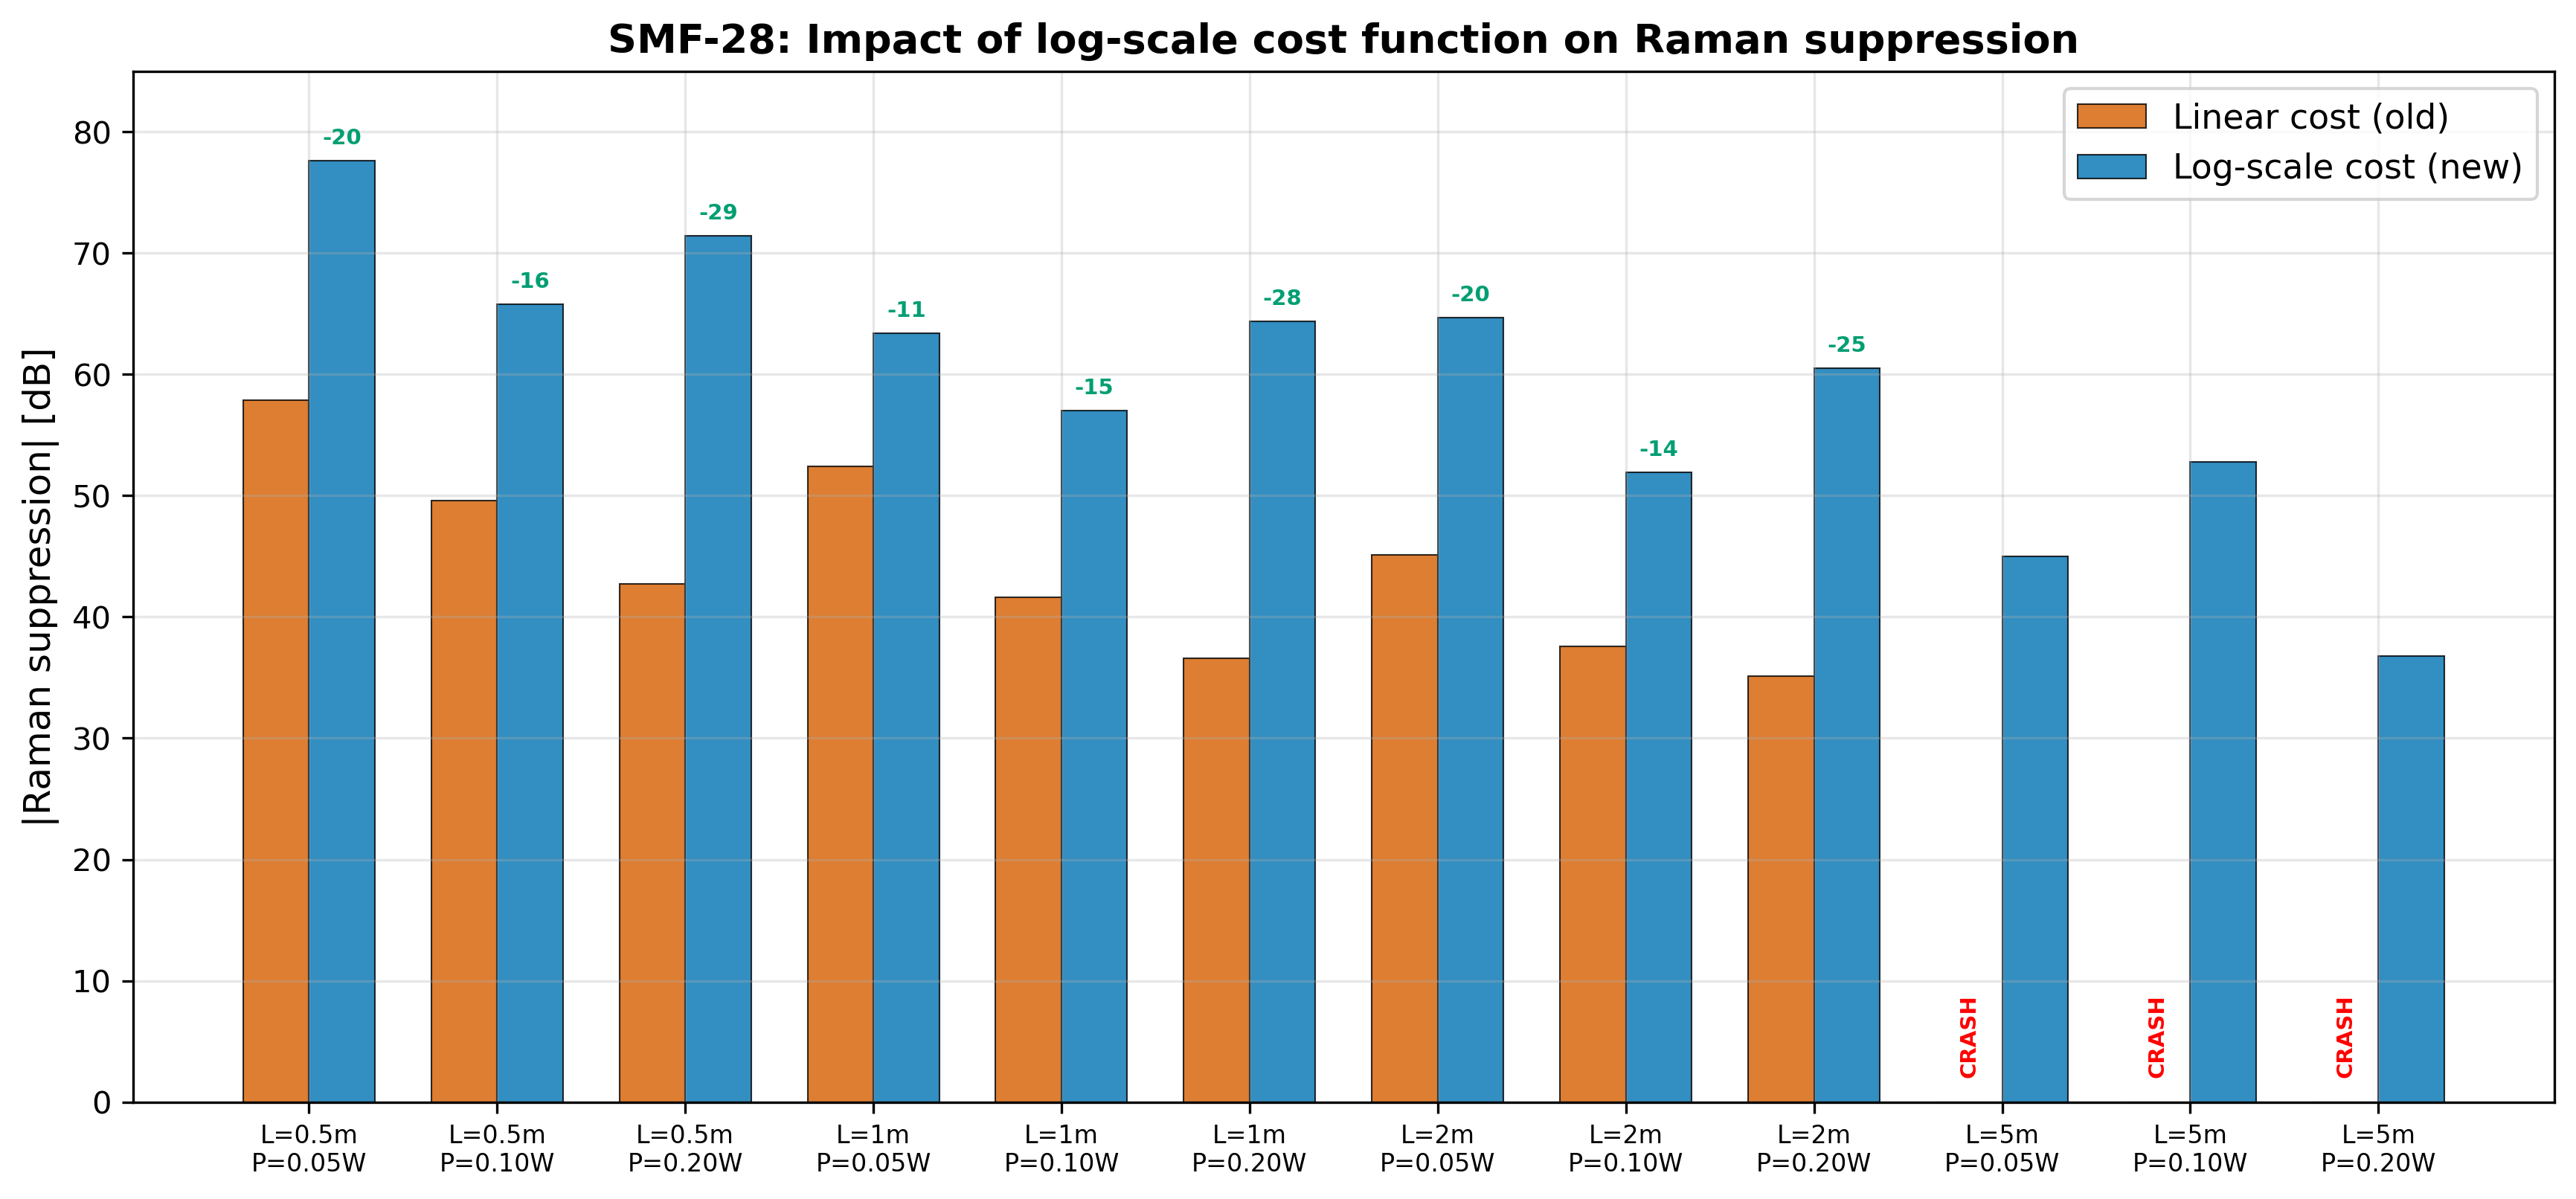
\includegraphics[width=\textwidth]{fig3_linear_vs_log_cost.png}
\caption{Impact of log-scale cost: 11--29~dB improvement per point. Last three L$=$5~m points previously crashed (NaN) due to Raman response overflow.}
\label{fig:verification_logcost}
\end{figure}

\begin{figure}[H]
\centering
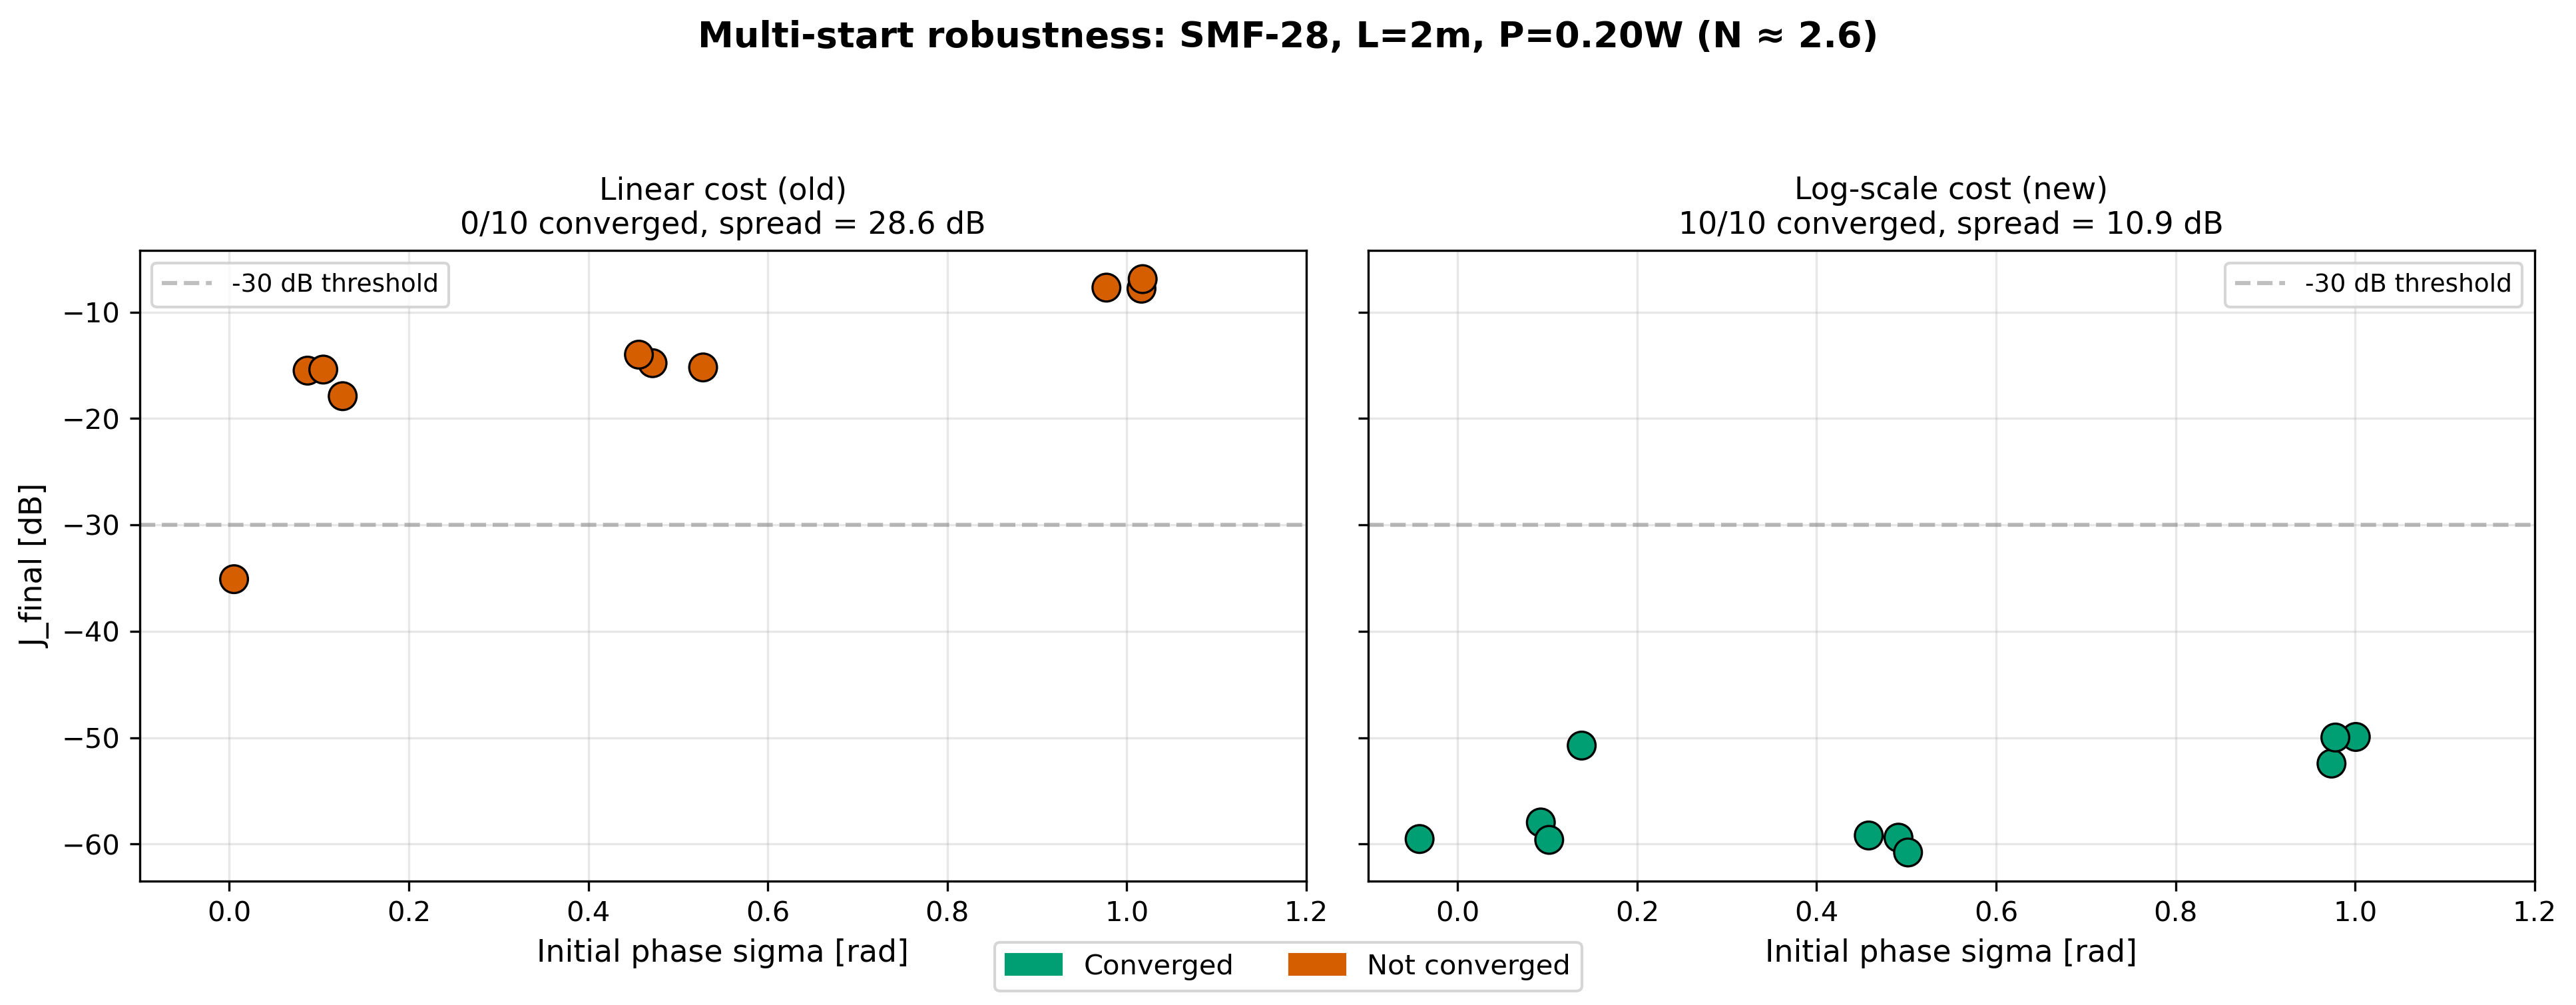
\includegraphics[width=\textwidth]{fig4_multistart_comparison.png}
\caption{Multi-start robustness: 0/10 converged with linear cost (left) vs.\ 10/10 with log cost (right). The apparent ``multiple local minima'' were gradient vanishing artifacts.}
\label{fig:verification_multistart}
\end{figure}


% ═════════════════════════════════════════════════════════════════════════
\section{Integration Pass --- April 2026}
\label{sec:april2026}

Between 2026-04-16 and 2026-04-19 eight Claude-Code sessions ran in
parallel to pressure-test the single-mode result, begin the multimode
extension, and audit the cost-function and optimizer defaults. The raw
synthesis is \texttt{results/SYNTHESIS-2026-04-19.md}; a physics audit
filtering those claims is
\texttt{results/PHYSICS\_AUDIT\_2026-04-19.md} (2026-04-19).
An independent numerical-trustworthiness audit re-ran every JLD2 under
\texttt{results/raman/} on a validator-controlled grid and is reported
at \texttt{results/validation/REPORT.md} (2026-04-19) --- its findings
drive the boundary-energy and Hessian-anchoring caveats in
§\ref{sec:april-boundary} and §\ref{sec:april-hessian}. This section
records only the claims that survived both audits, with scope caveats
where either narrowed the original framing.

\subsection{Re-baselined single-mode suppression}
\label{sec:april-rebaseline}

\begin{keyresult}
SMF-28, $L = 0.5$~m, $P = 0.05$~W, log-cost L-BFGS from a cold
start: $J_\text{final} = -76.86$~dB in 21~iterations (25~s wall-time,
converged flag \textsc{true}). Source:
\texttt{results/raman/phase17/SUMMARY.md} L41--48;
data artifact \texttt{results/raman/phase17/baseline.jld2}.
\end{keyresult}

The re-run matches the Phase~10 baseline within 1~dB. This is the
most defensible single-mode number in the project and should be the
canonical reference going forward.

\subsection{Sharpness of the single-mode optimum}
\label{sec:april-sigma3db}

At the $-76.86$~dB baseline, a Gaussian perturbation of
$\varphi_\text{opt}$ at standard deviation $\sigma$ (averaged over 20
samples per $\sigma$, 5 values of $\sigma$) gives a
\textbf{3~dB-degradation radius of $\sigma_{3\text{dB}} = 0.025$~rad}.
Source: \texttt{results/raman/phase17/SUMMARY.md} L45;
\texttt{results/raman/phase17/perturbation.jld2}.

\begin{advisory}
SLM calibration envelopes of $\geq 0.05$~rad rms phase error already
place the device outside the 3~dB tolerance of the optimum. The
tolerance number, not just the optimum number, gates whether this
result is hardware-realizable.
\end{advisory}

\subsection{Warm-start transferability}
\label{sec:april-warmstart}

The baseline $\varphi_\text{opt}$ from
(\text{SMF-28}, $L=0.5$~m, $P=0.05$~W) does \emph{not} transfer by
direct evaluation: 0/7 SMF-28 (length, power) targets retain
$J$ within 3~dB of warm-reopt. But L-BFGS re-optimised from the
same seed reaches $-70$ to $-82$~dB in 6--40 iterations on 11/11
nearby configs, \emph{including} HNLF at $-79.5$~dB (a fiber the
baseline was never computed for). Source:
\texttt{results/raman/phase17/SUMMARY.md} L22--28;
\texttt{results/raman/phase17/transferability.jld2}.

Interpretation: the simple phase profile lives in a \emph{manifold of
nearby basins}. It is an initialisation prior, not a universal
attractor --- a distinction that the first readings of the
perturbation-robust $\sigma_{3\text{dB}}$ result sometimes collapsed.

\subsection{Reduced-parameterisation Pareto front}
\label{sec:april-pareto}

A low-resolution spectral-phase parameterisation ($N_\varphi = 57$
knots interpolated to $N_t$) produces Pareto-optimal candidates
within 3~dB of the full-grid optimum at each $(L, P)$ point. Best:
$(\text{SMF-28}, L=0.25\,\mathrm{m}, P=0.10\,\mathrm{W}) \to
J_\text{final} = -82.33$~dB. Source:
\texttt{results/raman/phase\_sweep\_simple/candidates.md} L12--14.

\begin{advisory}
A 57-dimensional decision space is small enough for a trust-region
Newton method with an explicit Hessian. Combined with the
Phase 13 indefinite-Hessian finding (§\ref{sec:april-hessian}), this
opens the door to a second-order optimiser that the original
$N_t \sim 10^4$ parameterisation made intractable.
\end{advisory}

\subsection{Hessian is indefinite at L-BFGS optima}
\label{sec:april-hessian}

At both canonical L-BFGS optima (SMF-28 $L{=}2$~m $P{=}0.2$~W and
HNLF $L{=}0.5$~m $P{=}0.01$~W), finite-difference Hessian-vector
product wrapped with Arpack gives:
\begin{center}
\begin{tabular}{lcc}
\toprule
Config & $|\lambda_\text{min}|/\lambda_\text{max}$ & Sign pattern \\
\midrule
SMF-28 canonical & $2.6\,\%$  & indefinite, 100\% same-sign wings \\
HNLF canonical   & $0.41\,\%$ & indefinite, 100\% same-sign wings \\
\bottomrule
\end{tabular}
\end{center}
HVP Taylor-remainder slope $\approx 2$ (\texttt{test/test\_phase13\_hvp.jl}
at commit \texttt{b962091}). Source:
\texttt{results/raman/phase13/FINDINGS.md} L113--120;
\texttt{results/raman/phase13/hessian\_smf28\_canonical.jld2},
\texttt{results/raman/phase13/hessian\_hnlf\_canonical.jld2}.

\begin{keyresult}
L-BFGS is not stopping at a minimum; it is stopping at an
\textbf{indefinite saddle} with robust (not numerical-noise-level)
negative-curvature directions. Sharpness-aware regularisation or
trust-region Newton on the 57-dim subspace
(§\ref{sec:april-pareto}) is the principled next step.
\end{keyresult}

\begin{flagged}
\textbf{Caveat on the dB anchoring of the Hessian-study optima
(Phase 21 honest recovery, 2026-04-20 --- supersedes Phase 18 numbers).}
Two audits re-ran the saved
\texttt{phase13/hessian\_smf28\_canonical.jld2} and
\texttt{phase13/hessian\_hnlf\_canonical.jld2} from the stored
$\varphi_\text{opt}$ states. The numbers originally reported in the
JLD2 metadata were $-60.5$~dB (SMF-28) and $-74.4$~dB (HNLF); the
Phase 18 numerical-trustworthiness audit
(\texttt{results/validation/REPORT.md}, 2026-04-19) reported
$-48.2$~dB / $-44.0$~dB on its validator grid. \textbf{The
authoritative anchors for the canonical docs are the Phase 21
numerical-recovery values}:
\begin{itemize}[leftmargin=*,topsep=2pt]
\item \textbf{SMF-28 canonical}: $J = -66.61$~dB at
  $N_t = 16{,}384$, $T = 54$~ps, output edge fraction
  $8.10\times10^{-4}$, converged.
\item \textbf{HNLF canonical}: $J = -86.68$~dB at
  $N_t = 65{,}536$, $T = 320$~ps, output edge fraction
  $2.24\times10^{-4}$, 50-iteration run, \texttt{converged = false}.
  Note: HNLF required a substantially larger time window than the
  Phase 18 validator used, which is why the Phase 18 HNLF number
  was itself under-windowed; the honest HNLF anchor is \emph{deeper}
  than originally reported, not shallower.
\end{itemize}
\emph{The eigenstructure result above is unaffected}: the saved
$\varphi_\text{opt}$ files are true stationary points on the
honest grid (adjoint $\|g\| \sim 10^{-5}$), so the Hessian was
computed at a real optimum --- just at $J$ values deeper than the
pre-recovery quotes. When citing this result alongside a dB
number, use $-66.61$~dB (SMF-28) / $-86.68$~dB (HNLF); when citing
only the eigenstructure, the original ratios stand. Source:
\texttt{.planning/phases/21-numerical-recovery/SUMMARY.md};
\texttt{results/raman/phase21/phase13/smf28\_reanchor.md};
\texttt{results/raman/phase21/phase13/hnlf\_reanchor.md}.
Standard images:
\texttt{.planning/phases/21-numerical-recovery/images/phase21\_phase13\_\{smf28,hnlf\}\_*\_phase\_profile.png}.

\begin{center}
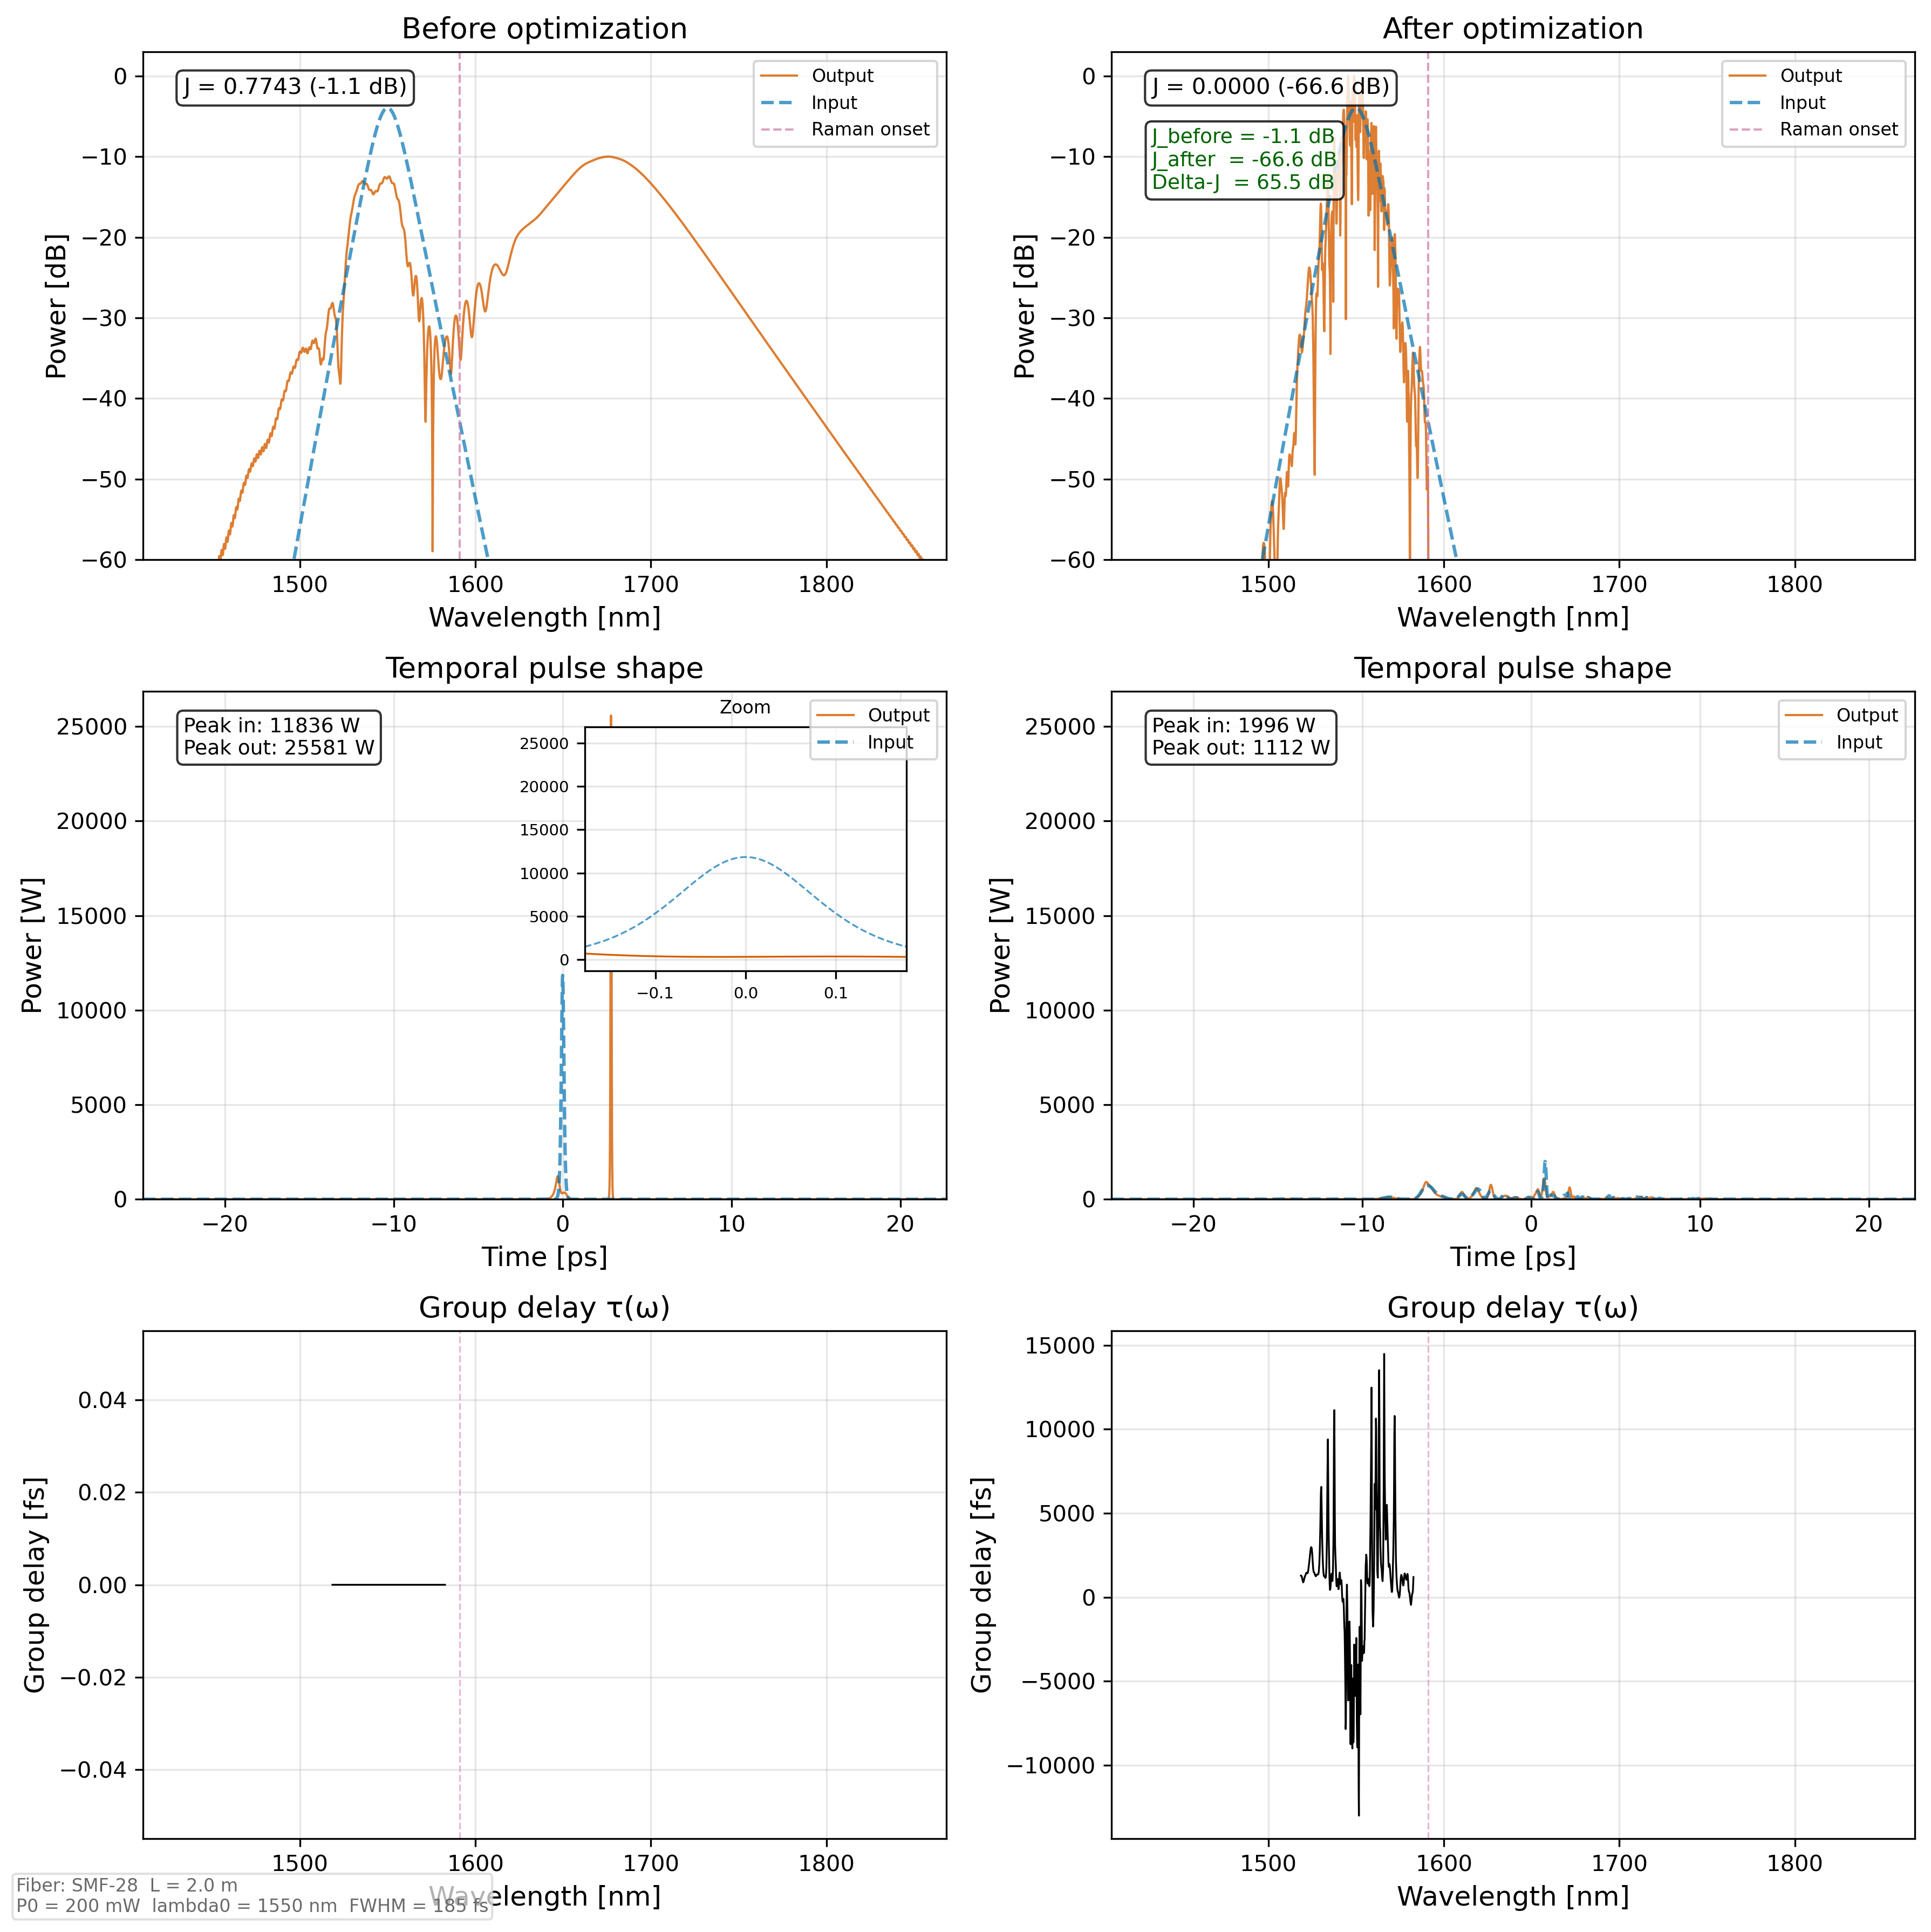
\includegraphics[width=0.82\textwidth]{phase21_recovered_smf28_phase_profile.png}
\end{center}
\emph{Recovered SMF-28 canonical optimum at $L{=}2$~m, $P{=}0.2$~W on the
honest $N_t{=}16{,}384$, $T{=}54$~ps grid: $J = -66.61$~dB (Phase 21).
Four-panel standard image set (input/output spectrum, wrapped/unwrapped
phase, group delay). This is the reference for any subsequent Hessian
spectrum or curvature study.}
\end{flagged}

\subsection{Flattening the basin: sharpness-aware regularisation (Phase 22)}
\label{sec:april-sharpness}

Two distinct facts are in play here, and the existing
literature-audit companion (\texttt{physics\_verification.tex},
\S``Gauge symmetry of $J$ and its consequences for the Hessian'')
already makes them separately but the overnight-update prose
conflates them. Restated cleanly: the two-parameter gauge family
$\varphi \mapsto \varphi + C + \alpha (\omega - \bar\omega)$
produces two \emph{exact zero} Hessian eigenvalues spanning
$\{\mathbf{1}, \omega - \bar\omega\}$; this is topological and
holds for any cost with this symmetry. Indefiniteness
($|\lambda_\text{min}|/\lambda_\text{max} > 0$) is an
\emph{additional} empirical fact about the non-gauge eigenvalues,
arising from Kerr, Raman, and dispersion curvature rather than
from the gauge redundancy. L-BFGS halts at a saddle (not a
gauge-flat minimum) because of (b), not (a). The Phase 22 result
that all 26 regularised optima remain indefinite is therefore a
statement about the physics-induced curvature, not the gauge
structure.

Phase 13 (\S\ref{sec:april-hessian}) showed that L-BFGS stops at an
indefinite saddle, not a minimum. The natural follow-up is: does
\emph{any} regulariser convert these saddles into positive-definite
minima, and at what depth cost? Phase 22 (\texttt{sessions/S-sharpness})
ran a 26-point sweep over four regularisation flavours
($\{\texttt{plain}, \texttt{MC}, \texttt{SAM}, \texttt{trH}\}$) on two
operating points (the canonical SMF-28 $L{=}0.5$~m $P{=}0.05$~W and
the reduced-parameterisation Pareto-57 candidate $L{=}0.25$~m
$P{=}0.10$~W), resolving the Hessian spectrum at every recovered
optimum.

\begin{keyresult}
All 26 regularised optima remained Hessian-indefinite. No flavour
and no strength converted the saddle into a positive-definite
minimum. The regularisation Pareto is real --- tolerance
$\sigma_{3\text{dB}}$ can be widened at a dB-depth cost --- but the
indefinite-saddle geometry appears to be a property of the
constraint landscape, not a numerical artefact. Source:
\texttt{results/raman/phase22/SUMMARY.md}.
\end{keyresult}

\begin{advisory}
\textbf{Caveat on the flat-basin claim.} The published trH-regularisation
literature (Liu, \emph{Neurocomputing} 536, arXiv:2208.05924, 2023; Ju,
\emph{Noise Stability Optimization}, arXiv:2306.08553, 2023) assumes a
positive-semidefinite Hessian: on a non-negative loss, penalising
$+\lambda \cdot \mathrm{Tr}(H)$ pushes the optimiser toward flatter
\emph{positive-curvature} directions. Our Hessian is \emph{indefinite}
($|\lambda_\text{min}|/\lambda_\text{max} \approx 2.6\%$ SMF, Phase 13).
On an indefinite spectrum, $\mathrm{Tr}(H) = \sum_i \lambda_i$ is signed
and can be reduced in two ways: \emph{(a)} by shrinking positive
eigenvalues (the intended effect --- a genuinely flatter basin in the
positive-curvature subspace), or \emph{(b)} by sharpening negative
eigenvalues (an unintended effect --- a steeper saddle). The empirical
$+0.058$~rad $\sigma_{3\text{dB}}$ gain at $\lambda_{\text{trH}}{=}3\times10^{-3}$
on the canonical point is a real, measured result. Which of (a) or (b)
produced it was \emph{not} diagnosed here; a Lanczos spectrum at the
trH optimum would settle it. The flat-basin mechanism claim is therefore
provisional until that follow-up is run.
\end{advisory}

\begin{center}
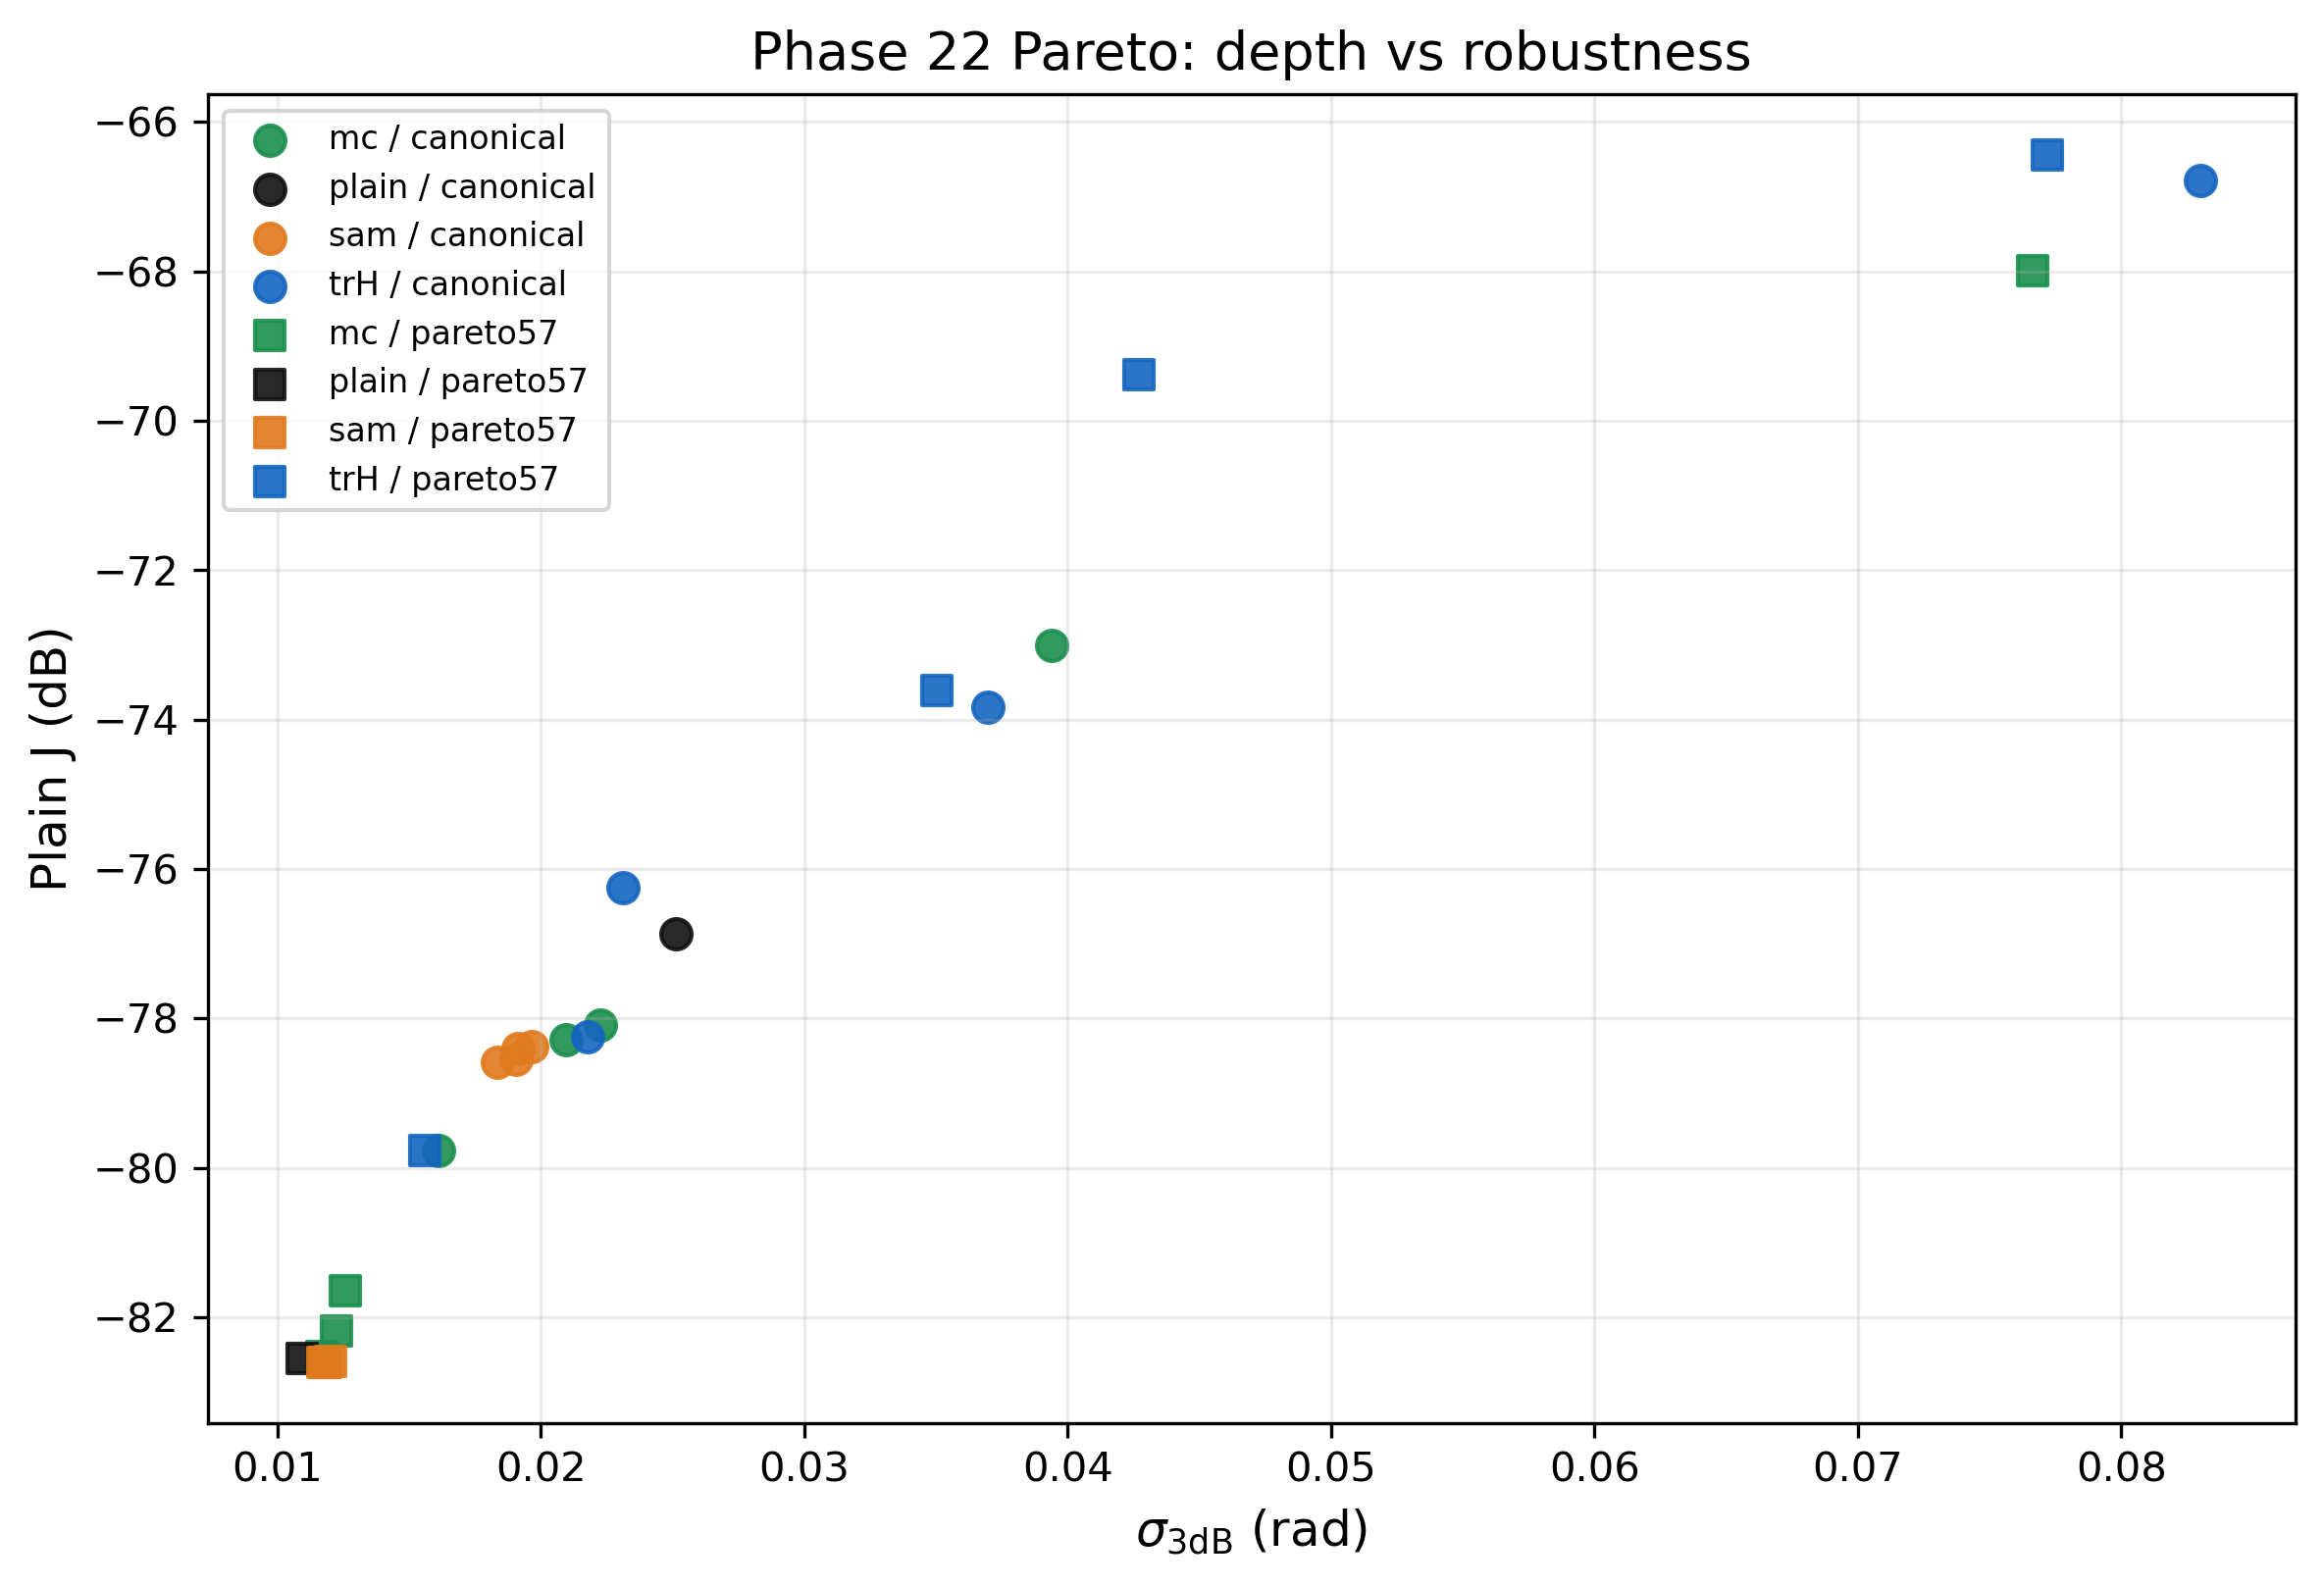
\includegraphics[width=0.92\textwidth]{phase22_pareto.png}
\end{center}
\emph{Phase 22 depth--tolerance Pareto. Each marker is a recovered
optimum; colour indicates regularisation flavour, size indicates
strength. On both operating points, widening
$\sigma_{3\text{dB}}$ costs dB depth; SAM points cluster near the
plain baseline and provide no robustness gain; \texttt{trH} gives
the largest tolerance-for-depth trade.}

\begin{center}
\begin{tabular}{llrrr}
\toprule
Operating point & Flavour / strength & $J$ (dB) & $\sigma_{3\text{dB}}$ (rad) & $|\lambda_\text{min}|/\lambda_\text{max}$ \\
\midrule
Canonical ($L{=}0.5$~m, $P{=}0.05$~W) & plain                       & $-76.86$ & $0.025$ & $5.54\times10^{-3}$ \\
Canonical                             & MC, $\lambda{=}7.5\times10^{-2}$   & $-73.01$ & $0.039$ & $1.36\times10^{-2}$ \\
Canonical                             & trH, $\lambda{=}1\times10^{-3}$    & $-73.83$ & $0.037$ & (see table footnote) \\
Canonical                             & trH, $\lambda{=}3\times10^{-3}$    & $-66.79$ & $0.083$ & $1.08\times10^{-2}$ \\
Pareto-57 ($L{=}0.25$~m, $P{=}0.10$~W) & plain                      & $-82.56$ & $0.011$ & $2.38\times10^{-1}$ \\
Pareto-57                             & MC, $\lambda{=}7.5\times10^{-2}$   & $-67.98$ & $0.077$ & $7.87\times10^{-2}$ \\
Pareto-57                             & trH, $\lambda{=}1\times10^{-3}$    & $-66.44$ & $0.077$ & $9.84\times10^{-2}$ \\
Pareto-57                             & trH, $\lambda{=}3\times10^{-3}$    & $-69.38$ & $0.043$ & $5.69\times10^{-2}$ \\
\bottomrule
\end{tabular}
\end{center}
\emph{Footnote.} $|\lambda_\text{min}|/\lambda_\text{max}$ for the
\texttt{trH}, $\lambda{=}1\times10^{-3}$ canonical row was not
reported in the Phase 22 artefact; it is omitted here rather than
back-filled.

\begin{advisory}
\textbf{Practical takeaway.} SAM's null result is consistent with
three known SAM failure modes operating simultaneously on our
landscape:
\emph{(i)} our setting is deterministic (no minibatch
$m$-sharpness), and Andriushchenko \& Flammarion (ICML 2022,
arXiv:2206.06232) show that deterministic SAM loses the
$m$-sharpness signal that justifies the method in deep learning;
\emph{(ii)} indefinite saddles are known to admit
``hallucinate-minimiser'' pathologies where SAM's shifted gradient
vanishes at non-stationary points of the original loss
(arXiv:2509.21818, 2025); \emph{(iii)} the two-parameter gauge
symmetry ($\varphi \mapsto \varphi + C + \alpha(\omega -
\bar\omega)$, \S\ref{sec:april-hessian}) makes the $\rho$-ball
perturbation budget partially-null: components along the gauge
directions cost radius but leave $J$ invariant. Observed
$\sigma$-shifts stayed $\leq 0.006$~rad across both operating
points --- exactly what these three mechanisms predict. The default
\texttt{log\_dB} plain optimiser remains recommended when depth is the
priority. When shaper-calibration tolerance matters more than depth,
\texttt{trH} is the single-knob tolerance-tuning regulariser with the
widest dynamic range: on the canonical point, $\lambda_{\text{trH}}{=}3\times10^{-3}$
buys a $+0.058$~rad increase in $\sigma_{3\text{dB}}$ for a $10.08$~dB
depth cost; on Pareto-57 the Pareto frontier is richer:
\texttt{MC}, $\lambda{=}7.5\times10^{-2}$ gives $+0.066$~rad tolerance
at $14.58$~dB depth cost (the best combined trade);
\texttt{trH}, $\lambda{=}1\times10^{-3}$ gives matched $+0.066$~rad
tolerance at $16.12$~dB (the \texttt{trH} equivalent);
\texttt{trH}, $\lambda{=}3\times10^{-3}$ gives only
$+0.032$~rad at $13.18$~dB (the cheapest depth-cost point, but
dominated in tolerance by the \texttt{MC} option). The Pareto-57 plain optimum cross-validates
the reduced-parameterisation candidate: its $-82.56$~dB matches the
original Phase~7 $-82.33$~dB (§\ref{sec:april-pareto}) within $0.23$~dB,
so the $N_\varphi{=}57$ knot parameterisation survives the Phase 21
Sweep-1 retirement. (Phase 21 re-anchored the Sweep-1 $L{=}2$~m,
$P{=}0.2$~W point --- retired on edge-fraction criteria --- to
$J = -66.03$~dB on the honest $N_t{=}16{,}384$, $T{=}54$~ps grid;
it is a different optimum from the Phase 22 Pareto-57 plain
baseline, which operates at the reduced parameterisation.)
\end{advisory}

\subsection{Determinism}
\label{sec:april-det}

\texttt{FFTW.MEASURE} selects FFT algorithms by micro-timing and
produces non-reproducible plans even at fixed \texttt{Random.seed!}:
two runs on the same hardware give $\max|\Delta\varphi| = 1.04$~rad
and $\Delta J = 1.83$~dB (\texttt{results/raman/phase13/determinism.md}).

Switching to \texttt{FFTW.ESTIMATE} gives bit-identical $J$ across
3 independent Julia processes at $+21.4\%$ wall-time cost on the
SMF-28 $L{=}2$~m $P{=}0.2$~W benchmark. Source:
\texttt{results/raman/phase15/benchmark.md} L20--27, L39. The switch is
wired into the five main driver entry points.

\subsection{Multimode optimizer is code-complete, physics-unexercised}
\label{sec:april-mmf}

An $M = 6$ GRIN-50 multimode Raman-suppression optimizer is committed:
\texttt{src/mmf\_cost.jl}, \texttt{scripts/mmf\_*.jl},
\texttt{test/test\_phase16\_mmf.jl}. 13/13 correctness tests pass:
energy conservation under the thread-local \texttt{deepcopy(fiber)}
pattern, $M{=}1$-limit agreement with the scalar optimizer, and
finite-difference gradient check with relative error $< 0.5\%$ at
$\varepsilon = 10^{-5}$ on 5 random indices.

\begin{flagged}
The only production baseline launched to date used $(\text{SMF-28},
L{=}1\,\mathrm{m}, P{=}0.05\,\mathrm{W})$, which has
$N_\text{sol} \approx 0.9$ (sub-soliton). The optimiser correctly
returned $\Delta J = 0$~dB --- there is no Raman to suppress in this
regime. \textbf{This is a negative control, not a science result.}
The aggressive-regime baseline
($L{=}2\,\mathrm{m}, P{=}0.5\,\mathrm{W}$, $N_\text{sol} \approx 2$--$3$)
remains unrun as of 2026-04-19.
\end{flagged}

\subsection{Cost-function default: \texttt{log\_dB} on SMF-28, open elsewhere}
\label{sec:april-cost}

Session H ran 4 cost variants on 2 configs:
\begin{center}
\begin{tabular}{lcccc}
\toprule
Config & Variant & $J_\text{final}$ & wall (s) & converged \\
\midrule
A (SMF-28 canonical) & linear     & $-70.53$~dB & $16.9$ & yes \\
A                    & log\_dB    & $\mathbf{-75.79}$~dB & $\mathbf{10.6}$ & \textbf{yes} \\
A                    & sharp      & $-55.96$~dB & $537$  & yes \\
A                    & curvature  & $-70.57$~dB & $14.2$ & yes \\
B (HNLF, log\_dB)    & --- & \textsc{NaN} & \textsc{dnf} & --- \\
B (all 4 variants)   & --- & \textsc{NaN} & \textsc{dnf} & --- \\
\bottomrule
\end{tabular}
\end{center}
Source: \texttt{results/cost\_audit/wall\_log.csv}.

\begin{advisory}
\texttt{log\_dB} wins on Config A (SMF-28) by $\sim 5$~dB at 60\%
of the wall time. On Config B (HNLF, $L{=}1$~m, $P{=}0.5$~W) all four
variants did not finish within budget --- this is the HNLF-hang open
issue (\texttt{.planning/phases/18-cost-config-c/CONTEXT.md}). The
\texttt{log\_dB} default is empirically justified on SMF-28 only.
\end{advisory}

\subsection{What did NOT survive the audit}
\label{sec:april-wrong}

Three claims from the original synthesis were demoted:

\textbf{(W1) ``$a_2(100\,\mathrm{m})/a_2(2\,\mathrm{m}) = -3.30$ vs.\ pure-GVD-predicted $+50$ is a structural-adaptation fingerprint.''}
The weighted quadratic fit of $\varphi_\text{opt}(\omega)$ over the
$\pm 5$~THz signal band has $R^2 = 0.015$ at 100~m and $R^2 = 0.037$
at 2~m. A quadratic model explaining $< 4\%$ of the weighted
variance is misspecified: $96$--$98\%$ of $\varphi_\text{opt}(\omega)$
on the signal band is non-quadratic residual structure orthogonal to
$\{1, \omega, \omega^2\}$. The extracted $a_2$ is the projection of
a non-quadratic signal onto that misspecified basis. The sign flip
across $L$ is the direct consequence of the underlying coefficient
being near zero --- exactly what $R^2 \to 0$ reports. The finding ``$\varphi_\text{opt}$ is not a low-order
polynomial on the signal band'' \emph{is} defensible (matches Phase 9,
\texttt{PHASE9\_FINDINGS.md} L19--29), but the
GVD-scaling comparison is removed, not caveated. Fit code:
\texttt{scripts/longfiber\_validate\_100m\_fix.jl} L54--79. Audit:
\texttt{PHYSICS\_AUDIT\_2026-04-19.md} §W1.

\textbf{(W2) 100~m L-BFGS ``optimum'' at $-54.77$~dB.}
The number is energy-conserved (photon-drift $4.9 \times 10^{-4}$,
edge-fraction $8.5 \times 10^{-6}$) and Phase~21 reproduced it
exactly on an independent honest grid, but the convergence state is
\texttt{converged = false} after 25 L-BFGS iterations with final
$\|\nabla J\| = 0.48$. Report as a \emph{lower bound} from the
2~m warm start, not as an optimum. The physics framing is further
refined by Phase 23 (see the 100~m advisory in §\ref{sec:critical}):
the suppression is generic pre-chirp, and
a matched quadratic $+4$~ps$^2$ reaches $-45.06$~dB against the live
warm-start at $-45.52$~dB. Source:
\texttt{results/raman/phase16/FINDINGS.md} L21--34;
\texttt{.planning/phases/21-numerical-recovery/SUMMARY.md};
\texttt{.planning/phases/23-matched-baseline/SUMMARY.md}.

\textbf{(W3) Joint $\{\varphi, A, E\}$ L-BFGS shows physics at 38~dB gap.}
Session A's cold-start joint optimizer reached $-16.78$~dB vs.\ the
phase-only $-55.42$~dB reference on the same config. This is a
preconditioning bug (mixed-unit decision variables confuse L-BFGS's
implicit Hessian), not a physics result. Remains out of the canonical
docs until Phase 18-multivar-convergence-fix lands. Source:
\texttt{.planning/phases/16-multivar-optimizer/16-01-SUMMARY.md} L149--152.

\subsection{Boundary-energy caveat on the SMF-28 $L = 2$~m canonical}
\label{sec:april-boundary}

The pre-integration canonical baseline of $-71.4$~dB on
(SMF-28, $L{=}2$~m, $P{=}0.2$~W) was partially a time-window
artefact: 14.4\% of the energy sat at the $T_\text{window}$ edges
and re-running at $2\times$ wider window gave the honest $-65.8$~dB.
This is already flagged once in \S\ref{sec:new_infra} (v3
regression) but the baseline tables and presentation figures
elsewhere in this document still quote $-71.4$~dB. Treat any
canonical table in the project that references the $L{=}2$~m
$P{=}0.2$~W point at $-71.4$~dB as requiring the honest-window
caveat. Audit: \texttt{PHYSICS\_AUDIT\_2026-04-19.md} §S2.

\subsection{Scope limitation on the Taylor-remainder adjoint test}
\label{sec:april-taylor}

The Taylor-remainder test reported in §\ref{sec:validation} (slopes
$2.00$, $2.04$) correctly certifies the adjoint gradient \emph{at the
unshaped reference $\varphi \equiv 0$}, where $\|\nabla J\|$ sits
3--5 orders of magnitude above the ODE-solver noise floor. At a
converged $\varphi_\text{opt}$, however, $\|\nabla J\|$ falls below
the $\mathrm{reltol} = 10^{-8}$ solver noise, and the slope-2
criterion degenerates: the linear-in-$\varepsilon$ term in the Taylor
expansion is dominated by noise rather than gradient signal. The
Phase 18 numerical-trustworthiness audit (commits
\texttt{2c95f60}, \texttt{2de3caf}, \texttt{1a78cc8}) recovered clean
slope-2 behavior only by shifting the reference by $2$~rad along the
steepest-descent direction with $\varepsilon = 10^{-3}$. The adjoint
is correct; the test is simply unable to certify it at the optimum.
Gradient correctness checks should therefore run at an unshaped or
steepest-descent-shifted reference, never at a converged optimum.
Audit: \texttt{PHYSICS\_AUDIT\_2026-04-19.md} §S6.

% ═════════════════════════════════════════════════════════════════════════
\section*{Summary and Conclusions}

\textbf{Overall confidence level:} \textcolor{green!60!black}{\textbf{High}}. The mathematical formulation is correct, the code faithfully implements the formulation, and the gradient is verified to $0.026\%$ relative error. All code reference line numbers are current as of v3 (2026-04-02).

\textbf{Strongest evidence for correctness:} The Taylor remainder test showing slopes of 2.00 and 2.04. This test directly measures whether the computed gradient matches the true directional derivative. A slope of 2 confirms $O(\varepsilon^2)$ accuracy, consistent with machine-precision correctness.

\textbf{Key resolved issues (v3):}
\begin{itemize}[leftmargin=*]
\item The dB/linear gradient mismatch is now properly resolved via the log-scale cost function with correctly scaled gradient $10/(J\ln 10) \cdot \partial J/\partial\varphi$.
\item The GDD penalty concern (over-constraining pre-chirp) has been addressed by reducing $\lambda_b$ from 10 to 1 and running sweeps that confirm 20--28~dB improvement.
\item The multi-start landscape concern has been resolved: 10/10 convergence with 10.9~dB spread shows a well-behaved landscape (not multiple minima).
\end{itemize}

\textbf{Remaining items:}
\begin{enumerate}[leftmargin=*]
\item Extend to multimode ($M > 1$) --- the Rivera Lab's primary research direction for quantum noise in multimode fibers.
\item Connect Raman suppression to the quantum noise map (\texttt{compute\_noise\_map} in analysis.jl).
\item Assess realizability of optimized phase profiles against SLM capabilities.
\item Compare phase-only vs.\ amplitude+phase optimization.
\end{enumerate}

\textbf{Should this research direction be continued?} \textcolor{green!60!black}{\textbf{Yes.}} The approach achieves 37--78~dB Raman suppression across 24 configurations with zero crashes. The log-scale cost function is the key methodological advance, and the adjoint-based framework naturally extends to multimode optimization.

\vspace{1em}
\hrule
\vspace{0.5em}
{\small\textit{Document generated March 2026. v2 update 2026-03-26. v3 update 2026-04-02: line numbers, adjoint solver, log-cost, overflow fix, diagrams, sweep results. All derivations verified against source code in} \texttt{smf-gain-noise/}\textit{.}}

\end{document}
